\documentclass[12pt,openany]{book}
\usepackage{lmodern}
\usepackage{setspace}
\setstretch{1.25}
\usepackage{amssymb,amsmath}
\usepackage{ifxetex,ifluatex}
\usepackage{fixltx2e} % provides \textsubscript
\ifnum 0\ifxetex 1\fi\ifluatex 1\fi=0 % if pdftex
  \usepackage[T1]{fontenc}
  \usepackage[utf8]{inputenc}
\else % if luatex or xelatex
  \ifxetex
    \usepackage{mathspec}
  \else
    \usepackage{fontspec}
  \fi
  \defaultfontfeatures{Ligatures=TeX,Scale=MatchLowercase}
\fi
% use upquote if available, for straight quotes in verbatim environments
\IfFileExists{upquote.sty}{\usepackage{upquote}}{}
% use microtype if available
\IfFileExists{microtype.sty}{%
\usepackage{microtype}
\UseMicrotypeSet[protrusion]{basicmath} % disable protrusion for tt fonts
}{}
\usepackage[left=4cm, right=3cm, top=3cm, bottom=3cm]{geometry}
\usepackage[unicode=true]{hyperref}
\hypersetup{
            pdfborder={0 0 0},
            breaklinks=true}
\urlstyle{same}  % don't use monospace font for urls
\usepackage{longtable,booktabs}
\usepackage{graphicx,grffile}
\makeatletter
\def\maxwidth{\ifdim\Gin@nat@width>\linewidth\linewidth\else\Gin@nat@width\fi}
\def\maxheight{\ifdim\Gin@nat@height>\textheight\textheight\else\Gin@nat@height\fi}
\makeatother
% Scale images if necessary, so that they will not overflow the page
% margins by default, and it is still possible to overwrite the defaults
% using explicit options in \includegraphics[width, height, ...]{}
\setkeys{Gin}{width=\maxwidth,height=\maxheight,keepaspectratio}
\IfFileExists{parskip.sty}{%
\usepackage{parskip}
}{% else
\setlength{\parindent}{0pt}
\setlength{\parskip}{6pt plus 2pt minus 1pt}
}
\setlength{\emergencystretch}{3em}  % prevent overfull lines
\providecommand{\tightlist}{%
  \setlength{\itemsep}{0pt}\setlength{\parskip}{0pt}}
\setcounter{secnumdepth}{4}
\usepackage[none]{hyphenat}
\usepackage[cmyk]{xcolor} % Recommended by US-AB
\usepackage{lmodern} % Recommended by US-AB
\usepackage{fancyhdr}
\usepackage{etoolbox}
\patchcmd{\chapter}{\thispagestyle{plain}}{\thispagestyle{fancy}}{}{} % Removes plain pagestyle from chapter headings (otherwise, page numbers are centered)
\AtBeginDocument{\addtocontents{toc}{\protect\thispagestyle{empty}}} 
\pagestyle{empty} % This makes ToC without header/footer
\usepackage[skip=15pt]{caption} % This should increase space below captions (not tested)
\raggedbottom
\usepackage[noindentafter]{titlesec}
\usepackage{titlesec}
\titleformat{\chapter}{\normalfont\bfseries}{\thechapter.}{15pt}{}\titlespacing*{\chapter}{0pt}{-50pt}{0pt}
\titleformat{\section}{\normalfont\bfseries}{\thesection.}{1em}{}\titlespacing*{\section}{0pt}{0pt}{0pt}
\titleformat{\subsection}[runin]{\normalfont\bfseries}{\thesubsection.}{1em}{}

\usepackage{CJKutf8} % For Mandarin in Acknowledgments

% For guiding quote in beginning of intro:
\makeatletter
% \renewcommand{\@chapapp}{}% Not necessary...
\newenvironment{chapquote}[2][2em]
  {\setlength{\@tempdima}{#1}%
   \def\chapquote@author{#2}%
   \parshape 1 \@tempdima \dimexpr\textwidth-2\@tempdima\relax%
   \itshape}
  {\par\normalfont\hfill--\ \chapquote@author\hspace*{\@tempdima}\par\bigskip}
\makeatother
\usepackage{placeins}
\usepackage{titlesec}
\newcommand{\sectionbreak}{\clearpage}
\usepackage{amsmath}
\usepackage{wrapfig}
\usepackage{caption}
\captionsetup[figure]{font=scriptsize}
\usepackage{float}
\usepackage{amssymb}
\usepackage{subcaption}

\author{}
\date{\vspace{-2.5em}}

\begin{document}

{
\setcounter{tocdepth}{4}
\tableofcontents
}
\cleardoublepage
\pagestyle{fancy} \fancyhf{} \renewcommand{\headrulewidth}{0pt}
\fancyfoot[LE,RO]{\thepage} \renewcommand{\floatpagefraction}{.9}
\setcounter{page}{9}

\chapter*{Abbreviations}\label{abbreviations}
\addcontentsline{toc}{chapter}{Abbreviations}

\begin{tabular}{ll}
\toprule
Abbreviation & Term\\
\midrule
mORF & main open reading frame\\
RPF & Ribosome Protected Fragment\\
TOP & Terminal oligopyrimidine\\
TE & Translation Efficiency\\
UTR & Untranslated region\\
uORF & upstream open reading frame\\
\bottomrule
\end{tabular}

\chapter{Introduction}

\section{Gene expression}\subsection{The central dogma of gene expression}

The whole genetic code of an organisms i stored as deoxyribonucleic acid
(DNA) molecules in a double stranded formation as chromosomes.
Chromosomes hold the DNA in a condensed state using chromatin, a complex
of DNA and proteins, structures. For transcription of DNA to occur
chromatin is remodeled to expose promotor regions in the DNA to which
fators assisting in transcription bind. One of these factors is DNA
polymerase that unravels the double-stranded DNA and creates a
single-stranded copy called ribonucleic acid (RNA) transcripts. This
copy is less stable due to its single strandedness and therefore only
temporary. The RNA transcripts undergo processing by which multiple
different transcript varaints coming from the same genomic region can be
produced. The protein coding portion of these transcripts are called
mRNAs. Once formed mRNAs are transported into the cytoplasm where they
are either degraded or associate with ribosomes. These ribosomes
translate the mRNAs into proteins by which the genetic information then
is expressed. Synthesised proteins, if no longer needed in the cell, can
be degraded by proteosomes (\textbf{see figure \ref{fig:geneExprPath}}).
This flow of genetic information into expressed proteins is commonly
referred to as the central dogma in molecular biology (F. Crick, 1970).

\clearpage

\begin{figure}
  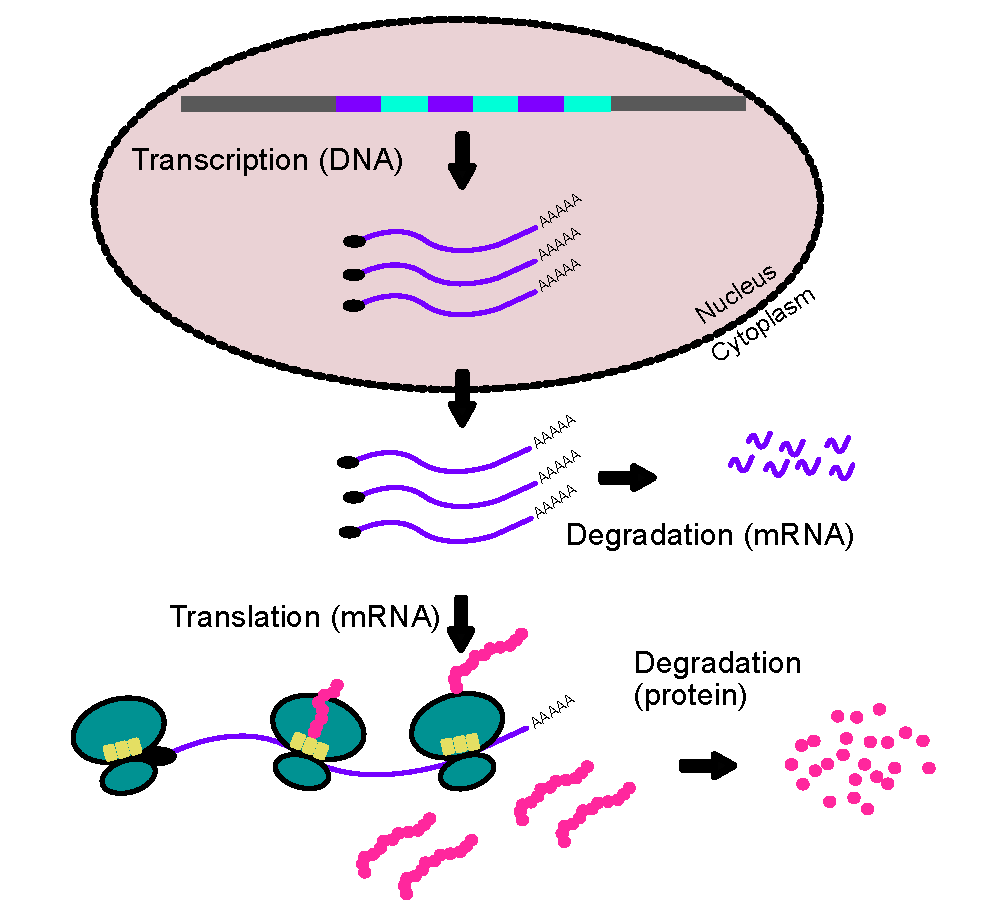
\includegraphics{./figures/geneExprPath_2.pdf}
  \caption{The gene expression pathway - DNA is transcribed in pre-mRNA containing a 5' cap (black oval) introns (teal boxes),exons (purple boxes) and a poly(A) tail. RNAs are processed into mRNAs consisting out ouf a 5' cap,exons and a poly(A) tail is then transported out of the cellular nucleus into the cytoplasm. Within the cytosplasm mRNAs can be degradated or translated  into proteins depending on cellular demands. Synthesised proteins can be degraded by proteosomes. \label{fig:geneExprPath}}
\end{figure}

\clearpage
\subsection{Contribution to gene expression} Proteins are the last
product of the gene expression pathway and carry out the vast majority
of all cellular functions. While it is apparent that modulation of
protein levels will offer information on the changes in gene expression,
it cannot completely answer the question as to why the levels change. In
a disease context, protein levels alone might offer sufficient insight
to explain phenotypic differences. However, how these differences arise
machanistically, which often poses as target for therapeutic strategies
in cancer, is obscured.

Experimental methods to measure gene expression at different steps are
often to referred as ``omics'' (i.e.~proteomics for protein expression,
transcriptomics for mRNA expression). These methods provide snapshots of
the step under scrutiny in a specific context (steady state or
perturbation) for a large portion of genes or proteins. Transcriptomics
studies approach gene expression with the assumption that mRNA
expression results in protein expression changes and can therefore be
used as a proxy. However, this view got challanged by landmark studies
that observed a poor mRNA to protein correlation and indicated a larger
role of post transcriptional regulation in gene expression than
previously assumed (J. Lu, Tomfohr, \& Kepler, 2005,Vogel \& Marcotte
(2012),de Sousa Abreu, Penalva, Marcotte, \& Vogel (2009),Schwanhäusser
et al. (2011),G. M. Silva \& Vogel (2016)).

The debate on which step of the gene expression pathway contributes most
is ongoing, nevertheless an understanding has been reached that the
cellular context is a major determinant. At steady state mRNA levels
seem to explain protein abundance best, however in perturbed systems the
contribution of transcript abundance is shifted away to other steps (Y.
Liu, Beyer, \& Aebersold, 2016). For example in a study that challanged
immune cells, protein levels were dependent on cellular transcript
levels (Jovanovic et al., 2015). In contrast a study investigating cells
under stress observed extensive modulation at the protein levels,
whereas mRNA transcript abundance was only mildly affected (Cheng et
al., 2016).

While the contribution of different steps of the gene expression is
dependent on many different factors, e.g.~cellular state or treatments,
mRNA translation (synthesis of proteins) is an essential process of this
pathway. Furthermore, dysregulation of mRNA translation has been
observed in a plethora of diseases, ranging from neurological disorders
to cancer which warrants for a comprehensive understaning of this
process (Kapur \& Ackerman, 2018,Ruggero (2013),L. J. Lee et al.
(2021),Graff et al. (2009)). This thesis will focus on the role of mRNA
translation in gene expression in the context of cancer. \clearpage

\section{mRNA translation}\subsection{Overview of an mRNA}

After transcription primary RNA transcripts are processed into mRNAs
which is the product that will be translated into proteins. The coding
region of an mRNA is flanked by untranslated regions (5' and 3' UTRs)
that exert translational control over the mRNA (see \ref{regmRNA}). The
5' has a cap that is important for mRNA translation initiation(Grifo,
Tahara, Morgan, Shatkin, \& Merrick, 1983), while the 3' end has a
poly-A tail protecting the mRNA against degradation (Wilusz, Wormington,
\& Peltz, 2001). Multiple different mRNAs (isoforms or transcript
variants) from the same genomic region exist. These variants can arise
due to a process called alternative splicing which alters the exon
composition (i.e.~coding region) of an mRNA. These variants can co-exist
at the same time and have distinct properties and can perform distinct
functions (Joly Anne-Laure et al., 2018).

\begin{wrapfigure}{o}{1\textwidth}
  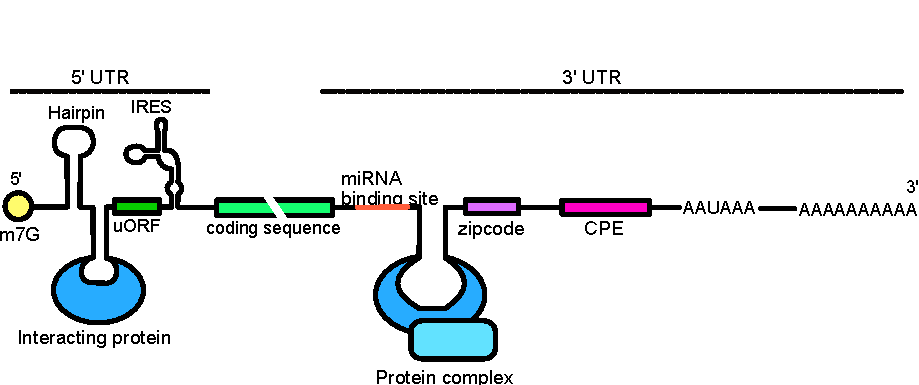
\includegraphics{./figures/UTRFeatures.pdf}
  \caption{ An mRNA consists of a coding sequence (green), 5' (light orange) and 3' (purple) untranslated regions flanking the coding sequence, a 5' cap and a poly-A tail. Located within the 5' and 3' untranslated region are cis elements (light red boxes) that can exert translational control by interfering with ribosomal movement along the mRNA or interact with trans factors (blue and red) or recruit the 43s ribsome (dark green) to the mRNA (see section \ref{regmRNA}). The codon composition of the coding sequence influences translation elongration rates (see section \ref{tRNA}).   
 \label{fig:UTRFeat}}
\end{wrapfigure}

\clearpage
\subsection{Translation of an mRNA} For the vast majority of protein
coding mRNAs, eukaryotic mRNA translation occurs in the cytoplasm,
however a small subset of mRNAs is translated in the mitochondria. mRNA
translation is a process that includes initiation, elongation,
termination and ribosome recycling and is an essential process
\textbf{see Figure \ref{fig:doodlemRNASteps}}. During the initiation
phase a ribome will associate with the mRNA and starts scanning along
the mRNA for a start codon to begin synthesis of the polypeptide chain
by incorporating amino acids. Amino acids are transferred to the
ribosome by specialised RNAs called transfer RNAs (tRNA) that can
recognise the genetic code in the mRNA. The availability of tRNAs as
well as their modification can influence the rate of elongation (see
\ref{tRNA}). The order by which amino acids are incorporated is dictated
by the order of the codons of the open reading frame (ORF). Redundancy
in the codon availability allows that amino acids are encoded by codons,
for example lysine is encoded by AAA and AAG. Once the ribosome
encounters a stop codon translation will terminate and the polypeptide
chain will be released. The ribosome then disassociates from the mRNA
and the ribosome can be recycled to engage translation of the same or
another mRNA. The following setions describe these processes in more
detail.

\begin{wrapfigure}{o}{1\textwidth}
  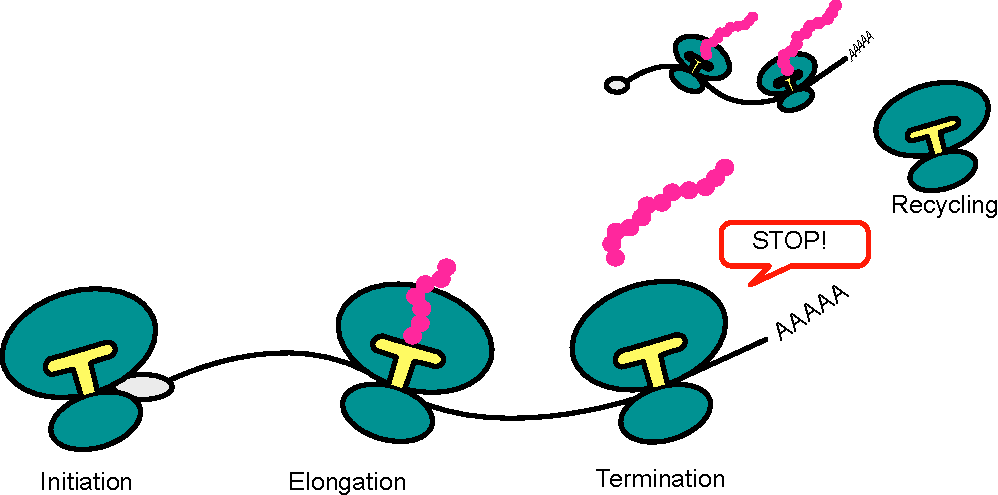
\includegraphics{./figures/doodleTranslation.pdf}
  \caption{mRNA translation initiation, elongation, termination and ribosome recycling steps - The ribosome binds to the mRNA and initiates scanning for a start codon. The elongation phase incorporates amino acids into a polypeptide chain (i.e. the protein product). Once the end of the coding sequence is detected, by recognition of stop codons, the ribosome terminates translation and releases the polypeptide chain. The ribosome can then be recycled to participate in the translation of another mRNA or reinitiate. \label{fig:doodlemRNASteps}}
\end{wrapfigure}

\clearpage

\subsection{Initiation} \label{initiation}

For the initiation to commence, in eukaryotes, two complexes are
required; the pre-initiation complex (PIC) and the eukaryotic initiation
factor 4F (eIF4F) complex. Both these complexes are governed by
signalling pathways that regulate their availability dependent on
cellular cues (\textbf{see section \ref{regmRNA}}). The PIC consists of
the methionyl-initiatior transfer RNA (met-tRNAi) in a ternary complex
(TC) with guanosine triphosphate (GTP) bound eIF2 (Asano, Clayton,
Shalev, \& Hinnebusch, 2000). eIF4F is the translation initation complex
containing three eIFs; eIF4E, the 5' cap binding protein, eIF4G a
scaffold protein and eIF4A and RNA helicase (Grifo et al.,
1983,Hinnebusch (2006)). eIF4F recruites the PIC to the 5' cap of the
mRNA after which scanning for a start codon (AUG) occurs. After AUG
recognition eIF2-GTP is hydrolyzed forming a stable 48S PIC.
Afterrelease of eIF2-GTP the 60S ribosomal subunit joins to form the 80S
ribosome and protein synthesis can start (\textbf{Figure
\ref{initiation}}).

\subsection{Elongation}

The 80S ribosome contains three sites important for decoding an mRNA;
the acceptor (A), peptidyl (P) and Exit (E) sites. During elongation in
eukaryotes aminoacytelated tRNAs are delivered to the A-site in a
ternary complex with eukaryotic elongation factor 1A (eEF1A). When the
tRNA recognises its cognate codon and pairs, a bond between the amino
acid and the polypeptide chain is formed. The formation of the bonds
causes the ribosomal units to rotate in relation to each other (Munro,
Altman, O'Connor, \& Blanchard, 2007,Moazed \& Noller (1989)). The
rotation causes a shift of the tRNA acceptor ends from the A and P to
the P and E sites, wheras the codon end remains in the A and P site.
This is the ``hyrbid'' state of the tRNAs in the ribosome(Dorner,
Brunelle, Sharma, \& Green, 2006). eEF2 then promotes the translocation
by which the codon ends of the tRNA follow into the P and E sites. The
deacytelated tRNA is then released from the ribosome. This process is
repeated until a stop codon (UAA, UGA or UAG) is detected by the
ribosome(C. U. T. Hellen, 2018){]}.

\begin{figure}[ht]
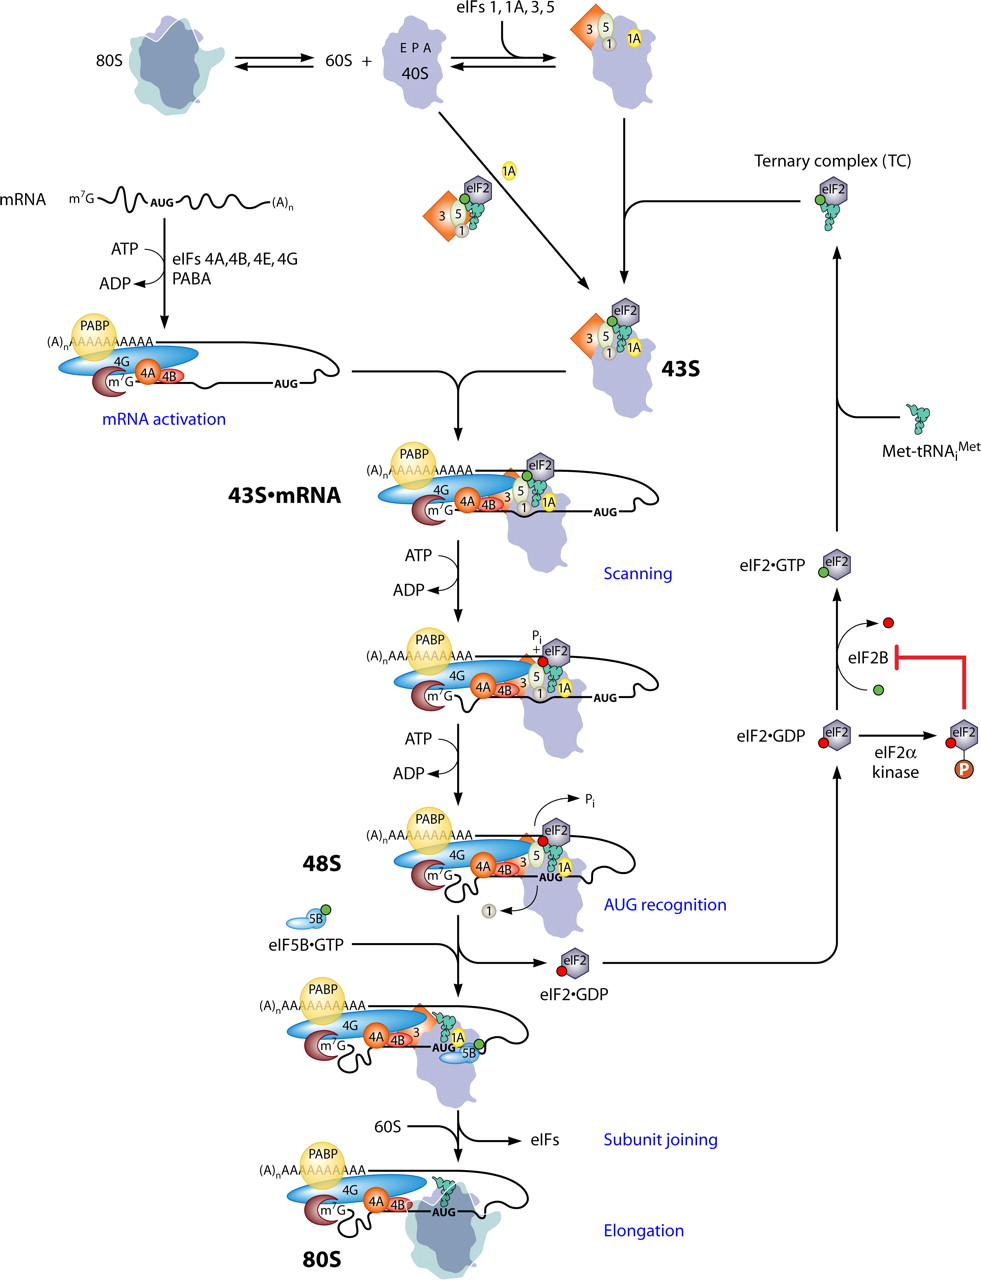
\includegraphics{./figures/initiation.jpg} 
  \caption{Pathway of eukaryotic translation initiation via ribosomal scanning.
  \label{fig:initiation}}
\end{figure}

\clearpage

\subsection{Termination and recycling}\begin{wrapfigure}{r}{.4\textwidth}
  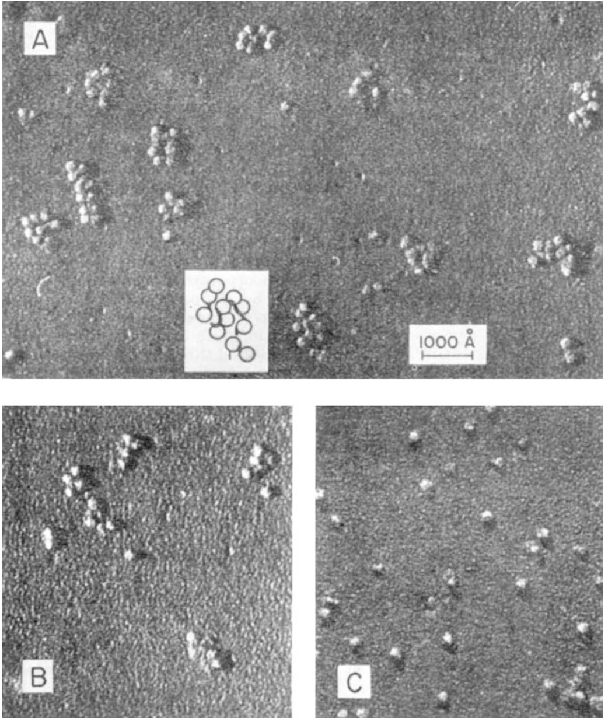
\includegraphics{./figures/polysome.pdf}
  \caption{Electromicrongraph of ribosomes extracted from different positions along a sucrose gradient used for polysome fractionation (A-C). For details on polysome fractionation see section \ref{exptMethod}. Reprinted with permission. DR. T. STAEHELIN et. al. Nature.1963 Aug 31;199:865-70.doi: 10.1038/199865a0. Copyright © 1963, Nature Publishing Group.
  Schematic of the TAPES method - A ribosome (A) can initiate with rate \(\alpha\) on an mRNA with a coding sequence with codons i= 1 ... L. The elongation rate at a specific codon is defined by \(\omega_i\) and \(\beta\) determines the termination rate once a stop codon is encountered. TASEP has been constantly modified, e.g. to allow for correction of initiation or elongation when the following codon is already occupied. Reprinted with permission. Juraj Szavits-Nossan and Martin R. Evans. 10.1103/PhysRevE.101.062404. ©2020 American Physical Society. 
 \label{fig:polysomes}}
\end{wrapfigure}

mRNa translation termination is facilitated by two eukaryotic release
factors (eRF), eRF2 and eRF3-GTP(I. Stansfield et al., 1995,Alkalaeva,
Pisarev, Frolova, Kisselev, \& Pestova (2006)). A TC containing eRF2 and
eRF3-GTP binds to the A-site of the ribosome upon recognition of a stop
codon. This causes an ATP hydrolysis event resulting in a conformational
change and release of the polypeptide chain. eRF1 and the ATP binding
cassette protein (ABCE1) together promote the splitting of the 60S and
40S subunits after which they can be recycled(Pisarev et al., 2010,Dever
\& Green (2012),C. U. T. Hellen (2018)).

\subsection{Translation efficiency}

Each ribosome synthesises a single protein during translation of an mRNA
assuming it is not prematurely terminated. It has been known since the
'60s that translation of an mRNA occurs via multiple bound ribosomes
(polysomes) simultaneaously (\textbf{see figure
\ref{fig:polysomes}A-C})(Warner, Rich, \& Hall, 1962,Staehelin, Brinton,
Wettstein, \& Noll (1963)).

The translation efficiency of an mRNA depends on the number of ribosomes
it is associated with synthesising proteins. While all steps of mRNA can
affect the translation efficiency of an mRNA, it is most commonly
regulated at the initiation step(Richter \& Coller, 2015,Dever \& Green
(2012),Jackson, Hellen, \& Pestova (2010)).

Assessment which step of mRNA translation is affected is often done
using experimental methods (e.g.~polysome profiling or by measuring
ribosome transit time). Furthermore, there are efforts to model
translation kinetics such as totally asymmetric simple exlcusion process
(TASEP) to obtain a better understanding of ribosome movements along the
mRNA (MacDonald, Gibbs, \& Pipkin, 1968,Maniloff (1969)) (\textbf{See
figure \ref{fig:polysomes}D}). A model that assessed ribosome traffic
under steady state and high initiation rates indicates traffic is not
only dependent on the densities of ribosomes but also condon specific
elongation rates and their distribution along the mRNA (Szavits-Nossan
\& Evans, 2020). The next section will go furhter into detail how mRNA
translation can be regulated so that intiation rates, but also
elongation, are influenced thereby altering translation efficiencies of
mRNAs.

\section{Regulation of mRNA translation} \label{regmRNA}

mRNA translation is the most energy consuming process in the cell, for
example in rat it was estimated to account for \textasciitilde{}20\% of
the cellular energy consumption (Buttgereit \& Brand, 1995). The role of
mRNA translation in gene expression and high energy consumption
therefore translational control is paramount, especially in cancer where
deregulated metabolism is common(Hanahan \& Weinberg, 2011).

A strong feature of translational control of initiation rates or
elongation rates is that it can affect mRNA distinct populations
differently. When one or more components of the translation machinery
are affected (e.g.~initiation factors, ribosomal proteins, tRNA
availability) translation of a large set of mRNAs is affected
(i.e.~global regulation). Whereas translational control acting on
characteristics of mRNAs, e.g.~through cis elements in the UTRs or RNA
binding proteins (RBP), selective regulation occurs. In some cases mRNAs
escape global translational control.

Major signalling pathways, e.g.~the PI3K/AKT/mTOR pathway and the
integrated stress response, regulate translation at a global level.
Furthermore, the codon usage of mRNAs can be used to regulate
translation globally dependent on the available tRNA pool or tRNA
modifications. Selective regulation of mRNA translation occurs via
characteristics a limitited population of mRNA share found in the 5' and
3' UTRs of an mRNA (Leppek, Das, \& Barna, 2018) (\textbf{see figure
\ref{fig:UTRFeat}}).

\subsection{mTOR} \label{mTOR}

mTOR is a conserved Ser/Thr kinase and is found in two structurally and
functionally distinct complexes, mTORC1 and mTORC2 (Saxton \& Sabatini,
2017,Pearce et al. (2007)). In a growth promoting environment mTOR
switches cell metabolism to increased production of protein, lipids and
nucleotides, while suppressing catabolic pathways. mTORC2 promotes
survival via signalling through protein kinase A (AKT) (Sarbassov,
Guertin, Ali, \& Sabatini, 2005).

mTOR activity is modulated via growth factor signalling (i.e.~insulin
and insulin-like growth factor; IGF1) as well as cellular metabolism.
Growth factor signalling es mediated through the phosphoinositide
3-kinase (PI3K) / AKT and Ras/mitogen-activated protein kinase (MAPK)
pathways. Both these signalling pathways are involved in oncogenic
signalling and under investigation as therapeutic targets in
cancer(Hilger, Scheulen, \& Strumberg, 2002,J. Yang et al. (2019)). In
several cancers (e.g.~breast, lung, prostate and colon) the gene
encoding the p110\(\alpha\) subunit of PI3K is frequently mutated or
amplified (D. A. Levine et al., 2005,Samuels et al. (2004),J. W. Lee et
al. (2005)). The E545K mutation which leads to a reduced inhibition of
p85 at the p110\(\alpha\) subunit (W. Jiang et al., 2018). In
\textbf{study 3} we investigate oncogenic signalling via the PI3K
pathway activated by insulin and the role of mTOR in mediating the
resulting effects on gene expression in the MCF7 breast cancer cell line
that harbours the E545K mutation (Schneck et al., 2013). Furthermore,
hyperactivity of PI3K/AKT and Ras/MAPK signalling pathways has been
reported in multiple cancers and been linked anti- cancer therapy
resistance (Pópulo, Lopes, \& Soares, 2012,Tan \& Yu (2013), Salaroglio,
Mungo, Gazzano, Kopecka, \& Riganti (2019)). mTOR, as a downstream actor
of these pathways integrating their singals, has therefore become a
focus of anti cancer therapy by either targetting mTORC1 or using dual
inhibitors for PI3K and mTOR (Bhat et al., 2015).

\begin{wrapfigure}{r}{0.6\textwidth}
  \includegraphics{./figures/mTORsignal.jpg}
  \caption{Schematic representation of mTOR signaling to the translational machinery. Philippe P. Roux, and Ivan Topisirovic Mol. Cell. Biol. 2018; doi:10.1128/MCB.00070-18. Reprinted with permission. Copyright © 2018, American Society for Microbiology
 \label{fig:mtorsignal}}
\end{wrapfigure}

mTOR fulfills a central role in metabolic signalling where it integrates
amino acids availability, glucose and cellular oxygen levels to form an
appropriate response. For example, amino acid availabilty induces
relocalisation of mTOR into proximity of Rag GTPases leading to its
activation (Sancak et al., 2008). Furthermore, Glucose deprivation and
oxygen availability regulate mTOR activity via adenosine-mono-phosphate
kinase (AMPK) signalling. AMPK is activated when a shift in the cellular
AMP to adenosine-tri-phophate (ATP) ratio is sensed (Sanders, Grondin,
Hegarty, Snowden, \& Carling, 2007,Kimball (2006)). While hypoxia,
deprevation of oxygen, inhibits protein synthesis in normal cells, in
breast cancer protein synthesis was not inhibited during hypoxia
attributed to uncontrolled mTOR signalling (Connolly, Braunstein,
Formenti, \& Schneider, 2006).

Given the central of mTOR governing proliferation, growth and
metabolism, which are often deregulated in cancer, it is vital to
comprehensively understand mTORC1 signalling herein (Hanahan \&
Weinberg, 2011).

\subsubsection{Global regulation of translation via mTOR}

mTOR regulates mRNA translation mainly by mediating availability of
eIF4E by phosphorylating 4E binding proteins (4E-BPs)(A.-C. Gingras et
al., 1999). eIF4E is required for mRNA 5' cap binding and formation of
the mRNA translation eIF4F complex. Therefore, inhibtion of mTOR leads
to a down regulation of cap dependent mRNA translation initiation. eIF4E
has overexpression is commonly found cancers and targetted using
4E-antisense oligonucleotides as anti-cancer therapy (D. S. Hong et al.,
2011). Other downstream targets of mTOR such as S6k which has been shown
to regulate components of the translation machinery, e.g.~by activiation
of programmed cell death protein 4(PDCD4) which disrupts eIF4G-eIF4A
binding through competition(, Dorrello et al., 2006,A. Göke et al.
(2002)).

\subsubsection{Selective or "mTOR sensitive" regulation of translation}

translation involves transcripts with a terminal oligo pyrimidine (TOP)
motif consisting of a C followed by a stretch of 4-15 pyrimidines
directly after the 5' cap show near complete dissociation from ribosomes
under conditions when mTOR is inhibited (Meyuhas, 2000,Yamashita et al.
(2008)). TOP mRNA are enriched for genes encoding for parts of the
translation machinery (Meyuhas, 2000,Thoreen et al. (2012)). Recent work
indicates the importance of La ribonucleoprotein domain family member 1
(LARP1) in regulation of TOPs. LARP1 is thought to bind to the 5' mRNA
cap of TOP mRNAs via its DM15 domain and represses translation by
obstructing eIF4E binding. mTORC1 physically interacts and
phosphorylates LARP1. When phophorylation occurs close to the DM15
domain of LARP1 the inhibitory effect on mRNA translation of TOP mRNAs
is abolished (Jia et al., 2021). Other instances of selective
translation are for mRNAs that lack the TOP motif, but show sensitivity
to mTOR activity. These mRNAs are, in addition to mTOR, dependent on
either availability of eIF4E or activity of eIF4A (\textbf{see
\ref{eif4a}}). mTOR-eIF4E sensitive mRNAs show extremely short 5' UTRs
and encode for metabolic functions(Gandin et al., 2016b).

\clearpage
\subsection{The integrated stress response} is a signalling pathway
which can be activated through kinase signalling orginating from various
stress signals. These kinases include Protein kinase R-like endoplasmic
reticulum kinase (PERK) which is activated by misfolded peptides in the
endoplasmatic reticulum (ER), Heme regulated eIF2alpha kinase (HRI)
which is activated during oxidative stress, protein kinase R (PKR) which
is activated in response to certain viral infections and GCN2 which is
activated when cells are deprived of amino acids(Kapur, Monaghan, \&
Ackerman, 2017,Guan et al. (2017),Taniuchi, Miyake, Tsugawa, Oyadomari,
\& Oyadomari (2016),Andreev et al. (2015)). During the integrated stress
response the alpha subunit of eIF2 is phosphorylated. Upon eIF2alpha
phosphorylation, eIF2 alpha directly engages the guanine nucleotide
exchange factor eIF2beta and precents conversion of inactive eIF2-GDP to
active eIF2-GTP needed for met-tRNAi incorpration in the TC, therefore
inhibiting translation by reducing PIC availability (Sonenberg \&
Hinnebusch, 2009) (\textbf{see also figure \ref{fig:initiation}}).

\subsubsection{Global and selective regulation of translation via the ISR}

is, similar to mTOR signalling, achieved at a global and selective mRNA
level. Phosphorylation of eIF2 alpha limits ternary complex
availability, therefore ribsome recruitment to the 5' cap is limited
which results in a reduction of translation initiation. While global
translation is reduced upon ISR, translation of a selective subset of
mRNA with upstream open reading frames (uORFs) is increased. A uORF is a
reading frame that originates in the 5' UTR of an mRNA upstream of which
the AUG precedes that of the coding sequence. uORFs are out of frame
with the main ORF and when translated lower the expression of the
mORF(Kozak, 1984). Ribosome profiling studies indicate that 50\% of
mammalian mRNAs harbour uORFs including oncogenes and transcripts
important in differentiation and cell cycle (Calvo, Pagliarini, \&
Mootha, 2009,Ingolia, Lareau, \& Weissman (2011),D. R. Morris (1995)).
The surrounding context of the uORF is important for its inhibitory
effect through more efficient initiation, where the classical Kozak
context (i.e. {[}A,G{]}..\textbf{ATG}G) is most efficient(Kozak,
1986,Calvo et al. (2009)). ATF4, a transcription factor for stress
response genes, contains two uORFs of which one partially overlaps with
the mORF. Under normal conditions ATF4 mRNA translation is initiated at
uORF1 and reinitiation at uORF2 occurs. The close proximity of uORF2 to
the mORF causes ribosomes to scan past the mORF start thereby inhibiting
the translation of the coding sequence. Limitiation of TC availability
during ISR causes longer ribosome scanning times leading to that
ribosomes scan past uORF2 and initiate at the mORF(Pakos-Zebrucka et
al., 2016).

\subsection{Regulation of mRNA translation by tRNAs} \label{tRNA}

As touched upon earlier, tRNAs are an essential part of the translation
machinery that carry the amino acids, to be incorporated into the
polypeptide chain during the elongation process, to the ribosome. tRNAs
consist of a 76-90 long nucleotide sequence set into a ``cloverleaf''
structure forming several loops (Sharp, Schaack, Cooley, Burke, \& Soil,
1985) (** see figure tRNA**). The acceptor stem binds the amino acid
carried by the tRNA, while the anti-codon loop binds to the mRNA within
the ribosome via classical watson-crick pairing (Watson \& Crick, 1953).
Multiple codons can encode for the same amino acid (synonymous codons),
however the availability of the tRNAs for different codons may vary
which can influence elongation rates.

\begin{wrapfigure}{o}{0.6\textwidth}
  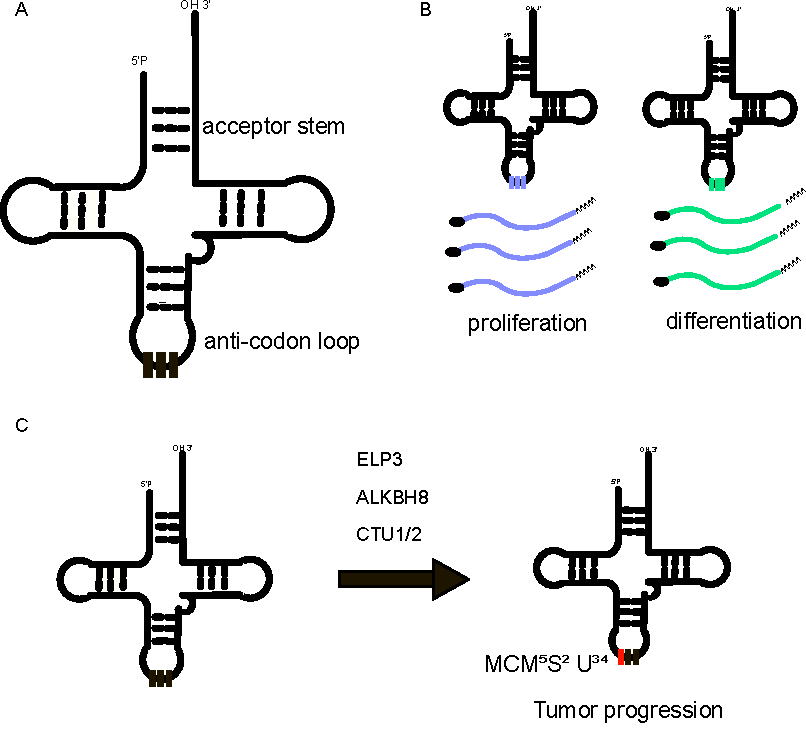
\includegraphics{./figures/tRNA.pdf}
  \caption{ (A) Schematic representation of the tRNA cloverleaf structure with indicated anti-codon and amino acid acceptor sites.  (B) Schematic representation of the proliferation and differentiation mRNAs dependent on distinct tRNA subsets. (C) Schematic representation of the U34 wobble position and the catalytic enzymes involved in this modifcation that is implied in tumor progression.
 \label{fig:tRNA}}
\end{wrapfigure}

This supply ( i.e.~tRNA availability) and demand (i.e.~codon in
expressed mRNA transcripts) relationship has been found to vary across
different cellular states, e.g.~profiferation and differentation. In
this model two distinct subsets of tRNAs are oberved; A tRNA subset
induced under proliferation that is otherwise repressed and a subset
with similar regulation under differentiation of which the supply
matches the codon demand of the transcriptome (Gingold et al., 2014).
Therefore, in this model differentiation and proliferation would underly
two distinct translational programs dependent on tRNA expression. This
model has been disputed and that the observed differences would be
attributed to GC content in the mRNA (Rudolph et al., 2016).
Nevertheless, abbarent tRNA expression and codon usage have been
reported in cancer(Z. Zhang et al., 2018). Furthermore, a comprehensive
study including small RNAseq (i.e.~for identification of tRNAs) and
protein samples across 17 tissues obtained from the The Cancer Genome
Atlas (TCGA) reported a tRNA signature stratified by Ki67 (a
proliferation marker) staining with implications for patient
survival(Hernandez-Alias, Benisty, Schaefer, \& Serrano, 2020).
Therefore, while a consensus on proliferation specific tRNA subsets
might not have been reached, emerging evidence implicates a role thereof
in cancer(Hernandez-Alias et al., 2020,Gingold et al. (2014),Z. Zhang et
al. (2018)).

Other reports of translational intereference by tRNAs in cacner are
attributed to tRNA modifications, specifically at the U34 anti- codon
(or wobble) position which is highly conserved (Rapino, Delaunay, Zhou,
Chariot, \& Close, 2017,El Yacoubi, Bailly, \& de Crécy-Lagard (2012)).
Wobbling was proposed by Francis Crick and refers to the ability of
non-watson-crick base pairing of tRNA anti codons(F. H. Crick, 1966).
This enables a smaller set of tRNAs (41-55 in eukaryotes) to encode for
the 64 possible codon combinations (Goodenbour \& Pan, 2006). In
mammals, the U34 modification catalytic cascade involves the
acetyltransferase Elongator (ELP3), the methyltransferase TRM9-like
domain of Alkylation repair homolog 8 (ALKBH8), and the urmylation (URM)
pathway, that includes the cytosolic thiouridylase homolog 1 and 2
(CTU1/CTU2)(Kalhor \& Clarke, 2003,Karlsborn et al. (2014)). These
enzymes ultimately modify the U34 modification into
5-methoxycarbonyl-methyl-2-thiouridine (\(mcm^5s^2U\)) which ensures
cognate codon recognition. This modification is thought to occur for a
small subset of tRNAs, namely \(tRNA^{UUU}\), \(tRNA^{UUC}\),
\(tRNA^{UUG}\), \(tRNA^{UCC}\), and \(tRNA^{UCU}\).

Loss of the ability to modify U34 has been shown to reduce translation
elongation rates with varying effects on protein expression (Nedialkova
\& Leidel, 2015,Deng et al. (2015),Zinshteyn \& Gilbert (2013)). While
in some cases U34 dependent signalling led to ribosome stalling
resulting in protein aggregates and increased stress (Nedialkova \&
Leidel, 2015,Zinshteyn \& Gilbert (2013)). Other reported a subtle
dowregulation of proteins encoded by mRNAs requiring U34-modified tRNAs
(Deng et al., 2015). U34 modifcation dependent tRNAs have been shown to
play a role in cancer. For example, ELP3 is important in tumor
initiation in the intestine and promotes breast cancer invasion as well
as progresstion to metastisis(Ladang et al., 2015,Delaunay et al.
(2016)). Furthermore, loss of U34 modification in a prostate cancer
model lead to an adaptive transcriptional response for mRNAs whose
translation was dependent on the U34 modification (Lorent et al., 2019).

\subsection{eIF4A sensitive mRNAs} \label{eif4a}

Progression of the ribosome through the 5' UTR is dependent on eIF4A,
the RNA helicase in the eIF4F complex, that unwinds structural elements
the ribsome encounters(Wolfe et al., 2014,Rubio et al. (2014)). The
importance of eIF4A's unwinding capacity was identified by treatment of
KOPT-K1 cells, a lymphoma cell line, MDA-MB-231 ,a breast cancer cell
line, with silvesterol of which translational control was evaluated
using ribosome prolfing (\textbf{see section \ref{riboseq}})(Wolfe et
al., 2014,Rubio et al. (2014)). These studies identified silvesterol
sensitive mRNAs that are characterised by long and structured 5' UTRs.
In addition eIF4A dependent mRNAs were enriched for having multiple 5'
UTR variants, while independet mRNAs were not (Rubio et al., 2014).
Among eIF4A dependent mRNAs are genes important for proliferation and
survival which has implications for oncogenic signaling(Wolfe et al.,
2014,Gandin et al. (2016b)). Among others, these studies indicate a
strong therapeutic value in targetting ``sensitive mRNAs'' in diseases.
In \textbf{study 2} we aimed to exploit eIF4A sensitve mRNA translation
as a theapeutic strategy in pancreatic cancer.

\subsection{RNA binding proteins and trans-acting factors}

The UTRs of an mRNA contain sequence elements to which RNA and RNA
binding proteins (RBPs) bind and exert translational regulation. For
instance, MicroRNAs, a small class of non coding RNA, can directly bind
to other RNAs and silence them accomplished through translational
repression or, more often, destabilisation {[}Jonas2015{]}. RBPs are a
class of proteins involved in many regulatory steps of gene expression
and account for \textasciitilde{} 7.5\% of the protein coding genes.
Poly-A-binding-protein (PABP) is thought to form a closed loop complex
of the 3' end to the 5' by interacting with eIF4G. This closed loop
should promote translation and prevent mRNA decay (Afonina, Myasnikov,
Shirokov, Klaholz, \& Spirin, 2014,Amrani, Ghosh, Mangus, \& Jacobson
(2008)) (\textbf{see also figure \ref{fig:initiation}}). An RBP of
particular interest in \textbf{study 3} is Human antigen R (HuR). HuR
preferentially binds to AU-rich sequences in the 3' UTR and acts as a
stabilizing agent and is involved in RNA-processing (T. D. Levine, Gao,
King, Andrews, \& Keene, 1993,Baou, Norton, \& Murphy (2011),X. C. Fan
\& Steitz (1998),S. S.-Y. Peng, Chen, Xu, \& Shyu (1998)). Studies in
breast, colon and lung cancer observed correlation between HuR and
malignancy. Among HuR targets are HIF-1, VEGF (important for
angiogenesis) and the oncogene Myc (Denkert et al., 2004,López de
Silanes et al. (2003),López de Silanes, Lal, \& Gorospe (2005)).

\section{Expertimental methods to measure mRNA translation} \label{exptMethod}\begin{wrapfigure}{r}{0.6\textwidth}
    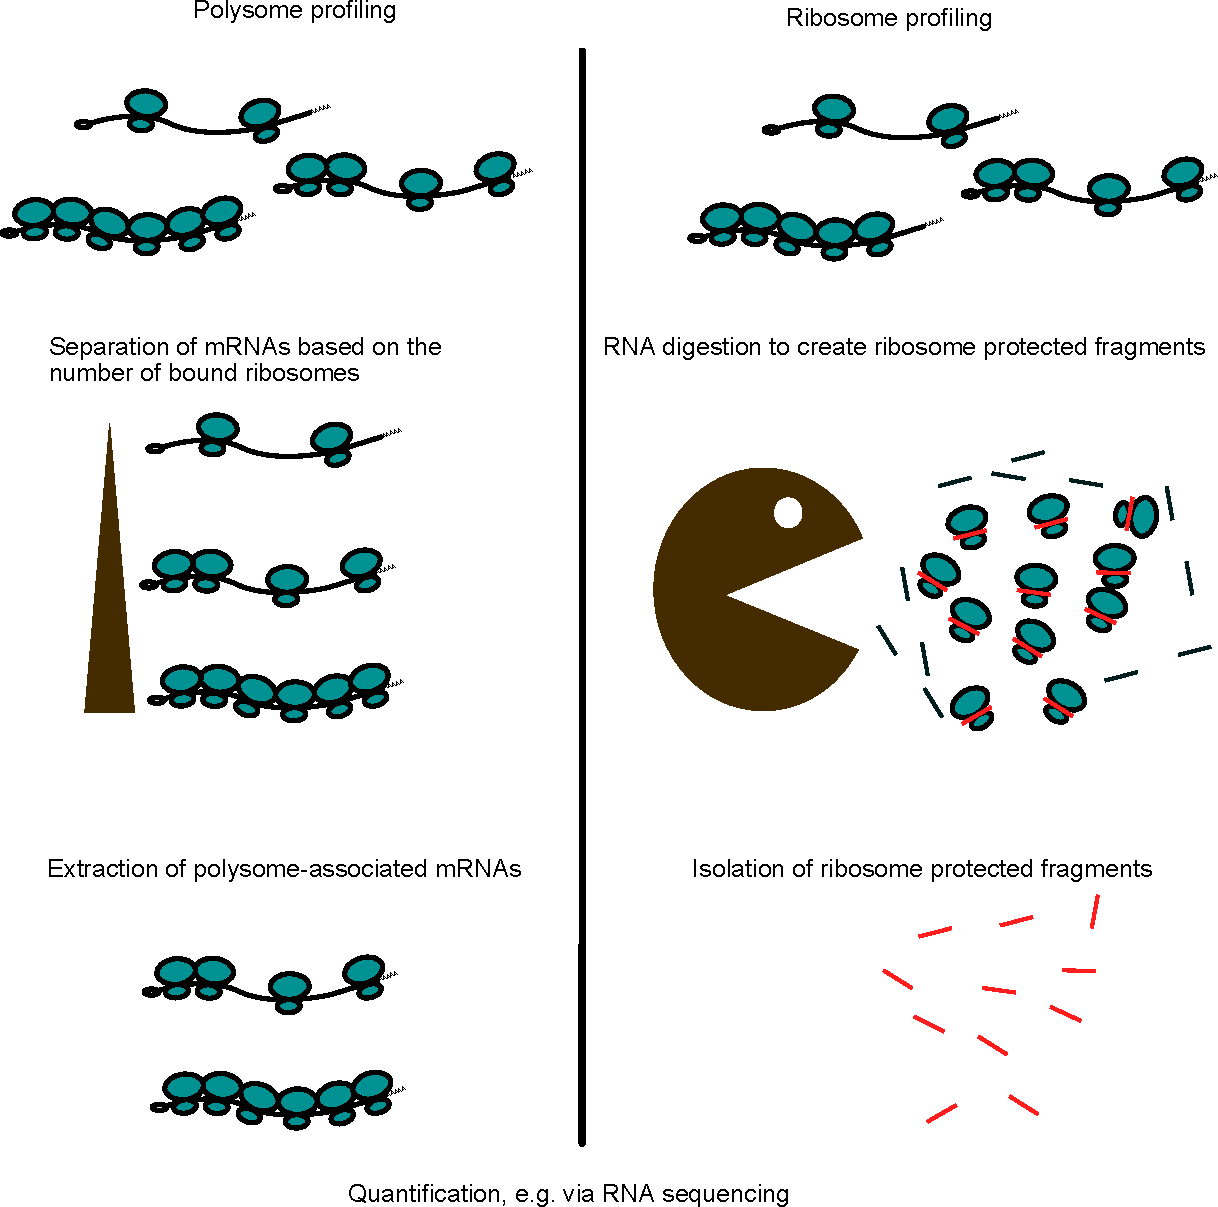
\includegraphics{./figures/polyRibo.pdf}
  \caption{Polysome profiling and ribosome profiling workflows. In polysome profiling a fraction from whole cytoplasmic RNA is loaded onto a sucrose gradient on which they get separated by sedimentation using ultra centrifugation. Fractions corresponding to efficiently translated mRNAs are collected and can be quantified with for example RNA sequencing (left). During ribosome profiling a fraction from the whole cytoplasmic RNA is exposed to a digestion agent which disturbs the RNA. The ribosomes will protect fragments thereby creating ribosome procted fragments. These fragments are then isolated and can be sequenced.  \label{fig:polyRibo}}
\end{wrapfigure}

Methods that measure mRNA translation try to capture the number of
ribosomes an mRNA is associated with on the prinicple that this is
directly correlated with their translation efficiency. There are two
methods that are predominantly used for measuring mRNA translation, or
changes in translation efficiencies across conditions, namely polysome
profiling and ribosome profiling (\textbf{see figure
\ref{fig:polyRibo}}).

\clearpage

\subsection{Polysome profiling}

is a technique to measure changes in translational efficiencies of mRNAs
between two or more conditions. Polysome profiling allows for separation
of polysomes from monosomes, ribosomal subunits and messenger
ribonucleoprotein particles (mRNPs). During the assay, ribosomes are
immobilized on the mRNAs using translation elongation inhibitors
(e.g.~cycloheximide). A portion of cytoplasmic RNA extracts are then
sedimented on a linear sucrose gradient (5-50\%) using ultra
centrifugation.

\begin{wrapfigure}{r}{0.6\textwidth}
    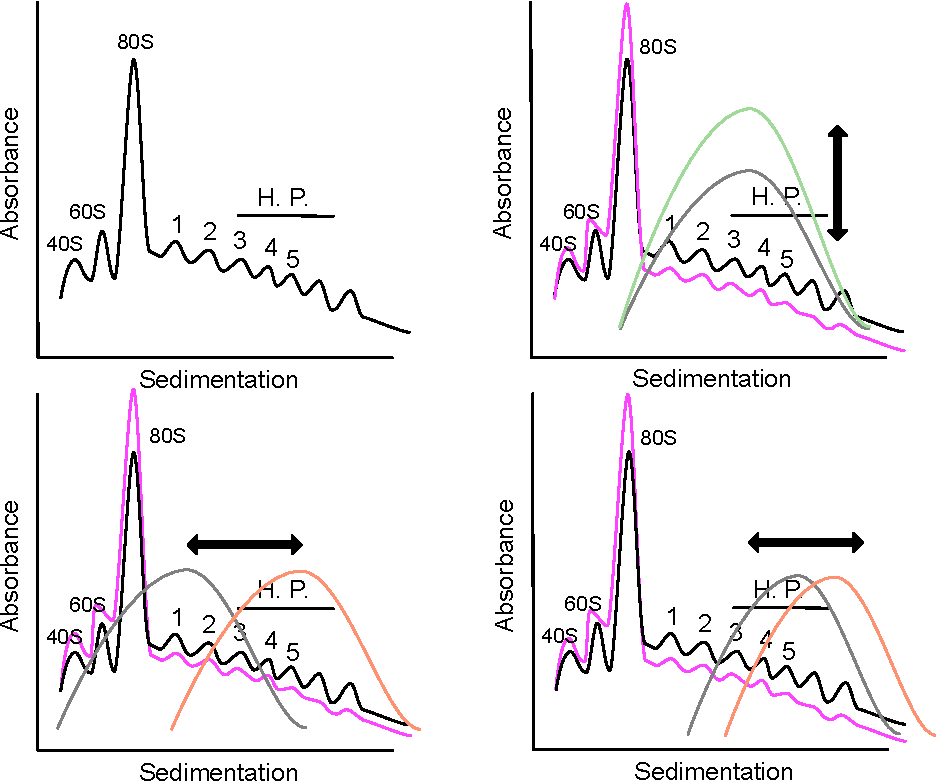
\includegraphics[width=0.9\linewidth]{./figures/polysome_shifts.pdf}
  \caption{Polysome profliles -  (top left) Schematic representation of a polysome profile using linear sucrose gradient fractionation. Indicated in the polysome profiles are the 40S, 60S ribosomal subunits as well as the 80S monosome. H.P. indicates heavy polysome fractions.Between conditions (i.e. black an pink lines) distribution changes for mRNA abundance (grey and green; top right), translation (grey and red; bottom left) and translation within high polysome fractions (grey and red; bottom right) are illustrated. \label{fig:polysome}}
\end{wrapfigure}

The resulting gradient is fractionated and mRNAs with different number
of bound ribosomes can be extracted and analyzed for changes in
translational efficiency (Gandin et al., 2014). An illustration of a
polysome profile with peaks for the 40S, 60S subunits and 80S ribosome
can be seen in (\textbf{Fig \ref{fig:polysome} top left}). Subsequent
peaks along the frations indicate the mRNAs with 1 or more bound
ribosome. mRNAs are typically normally distributed along the fractions,
i.e.~a pool of the same mRNA will be associated with 1- n number of
ribosomes. Changes in mRNA abundance will lead to an overall increase in
the amount of isolated polysome-associated mRNA without a shift of the
distribution along the fractions (\textbf{Fig \ref{fig:polysome} top
right}). This means that the translation efficiency per mRNA remains
unchanged. Changes in translational efficiency can be observed by shifts
of polysome association for mRNAs from the light (inefficiently
translated) towards the heavy (efficiently translated) polysome
fractions or vice versa (\textbf{Fig \ref{fig:polysome} bottom left}).
Shift within the heavy polysome fractions (i.e.~3 bound ribosome to 7
bound ribosome) can also occur (\textbf{Fig \ref{fig:polysome} bottom
right}). These shift remain undetected in cases where the distribtion of
polysome-associated mRNAs does not sufficiently shift across the
fractions and is a limitation of polysome profiling. Quantification of
mRNA levels within each fraction can be assessed using Northern blotting
or reverse transcription quantitative polymerase chain reaction
(RT-qPCR).

For transcriptome wide studies, pooling of efficiently translated mRNAs
(mRNAs with \textgreater{}3 bound ribosomes) followed by quantification
using either DNA-microarrays or RNA sequencing is common. The 3-ribosome
cut off has been chosen as it is thought to capture most biologically
relevant changes in translation efficiency. Pooling of mRNAs as well as
collection of multiple fractions makes polysome profiling inconvenient
when dealing with large samples sizes or experiments with low amounts of
input RNA. Therefore, an optimized sucrose gradient was developed where
most efficiently translated mRNAs are collected on a sucrose cushion and
thereby can be isolated from one single fraction (Liang et al., 2018).
This optimized gradient allows for application of polysome profiling in
small tissue samples where RNA quantity is limiting and reduces labor
intensity of the assay.

Polysome-associated mRNA levels are subject to changes in translation
efficiency as well as factors contributing to cytosolic mRNA levels.
Mechanisms such as transcription (i.e.~in the case of mRNA abundance) or
mRNA stability can affect cytosolic mRNA levels which impacts the pool
of mRNAs that can be associated to polysomes. Therefore, to identify
true changes in translation efficiency it is important to collect
cytoplasmic mRNA levels in parallel to polysome-associated mRNA to
correct for such mechanisms (e.g.~transcription or mRNA stability)
during downstream analysis (Gandin et al., 2014).

\subsection{Ribosome profiling} \label{riboseq}

Ribosome profiling is a technique that enables sequencing of ribosome
protected mRNA fragments (RPFs). In the assay ribosomes are immobilized
on the mRNAs using, similar to polysome profiling, translation
elongations inhibitors (e.g.~cyclohexamide) (Ingolia, Ghaemmaghami,
Newman, \& Weissman, 2009,Ingolia (2016)). One limitation with the use
of translation elongation inhibitors is the distortion of ribosome
distributions especially at translation initiation sites. These
introduced artefacts need to be accounted for in the downstream analysis
when assessing ribosome position along the mRNA. Following the
translation elongation inhibitor treatment, cells are immediately flash
frozen using liquid nitrogen. Alternatively, using only flash freezing
has been seen as a robust approach in a wide range of diverse organisms
(Brar \& Weissman, 2015).

RPFs are obtained by RNAse treatment that breaks the links of RNA
between ribosomes leaving single ribosomes with a \textasciitilde{}28
nucleotide long RNA fragment within each ribosome. The RPFs are then
isolated using ultra centrifugation through a sucrose cushion. During
this step other RNA fragments such as non-coding RNAs or large
ribonucleoprotein complexes can co-migrate and contaminate the sample.
Typically RPFs with a size randing from 25-30 nucleotides are selected
for quantification.

In parallel to RPF selection, randomly fragmented total mRNA of the same
size is also retrieved. This is achieved by extraction of total mRNA
from cell lysate followed by purification via recovery of polyadenylated
messages or removal of ribosomal RNA. (Ingolia et al., 2009,Brar \&
Weissman (2015)).

\subsection{Comparing ribosome and polysome profiling}

Albeit both methods generate count data after quantification with
RNAsequencing, there are some key aspects that differ between the
techniques. Polysome profiling separates efficiently translated mRNAs
from non- efficiently translated mRNAs along a sucrose thereby creating
an mRNA based perspective for analyzing changes in translational
efficiencies. In contrast, ribosome profiling determines translational
efficiencies by counting the number of RPFs of both efficiently and
non-efficiently translated mRNAs. This gives polysome profiling the
advantage in cases of transcript variants with important features in
their 5´UTR. Such information, if not protected by a ribosome, would be
lost in ribosome profiling.

Changes in translational efficiencies, e.g.~shifts between the polysomal
fractions, can be dramatic (I.e. near complete dissociation of ribosomes
from an mRNA) or subtle (shifts from 2 to 4 ribosomes) (Livingstone et
al., 2015). Ribosome profiling has been shown to be biased towards
identification of dramatic shifts of associated ribosomes to mRNAs,
whereas subtle shifts are masked which can lead to false biological
conclusions. Polysome profiling is affected by this to a much lesser
extent, thereby more robust in identifying such changes (Masvidal,
Hulea, Furic, Topisirovic, \& Larsson, 2017). Higher sensitivity in
detecting changes in translational efficiencies on a global scale makes
polysome profiling more suitable for genome-wide studies (Gandin et al.,
2016a).

An advantage of ribosome profiling is that it provides exact nucleotide
positions occupied by ribosomes. This offers information at a single
nucleotide level where the ribosome sits. Polysome profiling cannot
reveal ribosome locations along the mRNA. The single nucleotide
resolution of ribosome profiling is necessary in contexts studying local
translation events such as ribosomal frame shifts (Rato, Amirova, Bates,
Stansfield, \& Wallace, 2011) or uORF translation (Andreev et al.,
2015).

Both methods have their strengths and weaknesses and therefore each
method should be considered depending on the underlying biological
question of each experiment.

\section{Modes for regulation of gene expression in mRNA translation} \label{modes}

\begin{wrapfigure}{l}{0.6\textwidth}
  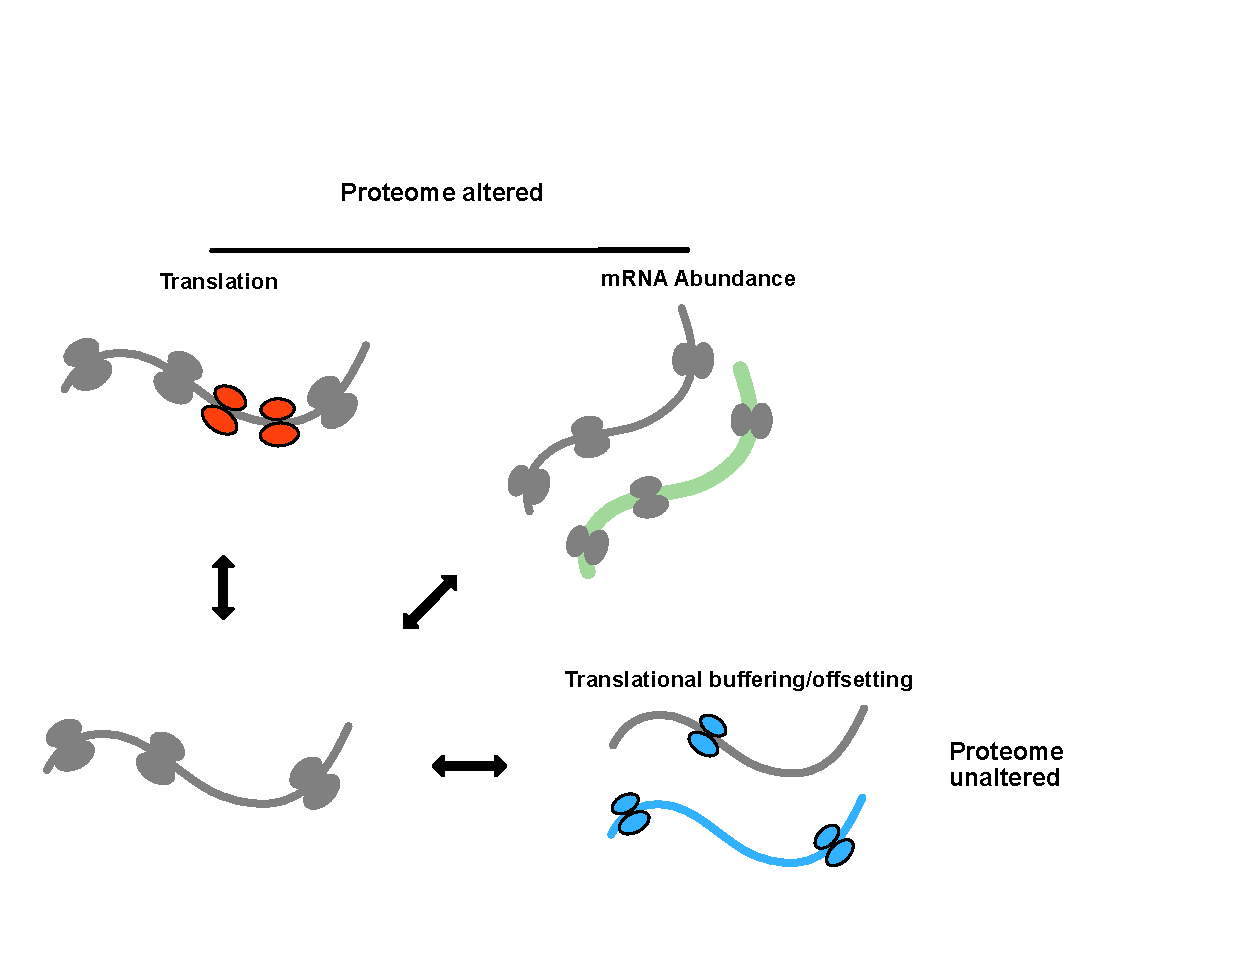
\includegraphics{./figures/geneModes_MRNA.pdf}
  \caption{Regulatory modes of gene expression - Schematic representation of regulatory modes of translation efficiency in a fold-change scatter plot. Indicated in red are changes in translation (i.e. changes in translated mRNA but not total mRNA), in green changes in mRNA abundance (i.e. congruent changes between total mRNA and translated mRNA) and in blue translational buffering (i.e. changes in total mRNA levels but not translated mRNA levels). TE changes as the TE-score would estimate them are indicated.\label{fig:modes}}
\end{wrapfigure}

As explained in the previous section, from genome-wide assessments of
translation using ribosome or polysome profiling expression levels for
both cytoplasmic and polysome-associated mRNAs (or RPFs). For the sake
of simplicity , from now on, these RNA types will be referred to as
total mRNA (i.e.~cytoplasmic mRNA) and translated mRNA
(i.e.~polysome-associated mRNA or RPFs). The estimation of expression
levels for both translated mRNA and total mRNA allows for interrogation
at two steps of the gene expression pathway and their interaction. The
interaction of total mRNA with translated mRNA can give valuable
insights for the underlying mechanisms that govern gene expression in
the studied system.

When comparing perturbed systems to their corresponding control state we
typically observe three ``modes'' in which translated mRNA and total
mRNA distinctly interact that impact gene expression (\textbf{See figure
\ref{modes}}). We refer to these modes as ``translation'', ``mRNA
abundance'' and ``translational buffering''.

\subsection{Translation}

A change in ``translation'' occurs when total mRNA levels remain
unaltered, however translated mRNA levels either increase or decrease
resulting in a change of their translation efficiency. A prominent
example of this mode can be observed to TOP mRNAs. These mRNAs, under
conditions when mTOR is inhibited, show a near complete dissassociated
from ribosomes(Gandin et al., 2016b). mRNAs under the translation mode
are expected to reshape the proteome (\textbf{See figure \ref{modes}}).

\subsection{mRNA Abundance}

Another mode that impacts the proteome is a change in mRNA abundance
which its concept is straight forward, here the translated mRNA level
changes to a similar magnitude as the total mRNA level. For these mRNAs
the translation efficiency is unaltered, as the change in total mRNA
levels explains the change in translated mRNA levels. Nevertheless,
since there are more (or less) mRNAs that are being translated an effect
the proteome is expected. The underlying biological implication for this
mode mRNAs is often related to transcription (\textbf{See figure
\ref{modes}}).

\subsection{Translational buffering} \label{modeBuffering}

In recent years, evidence emerged where translation efficiencies of
mRNAs can be altered to compensate for changes in total mRNA levels.
This mode is characterised by changes in total mRNA levels that are not
matched by translated mRNA levels. The expected result on the proteome
is that it maintaining (i.e.~keeping levels constant) rather than
reshaping it (McManus, May, Spealman, \& Shteyman, 2014,Lorent et al.
(2019)) (\textbf{See figure \ref{modes}}).

This mode was named ``Translational buffering'' and currently the
literature supports multiple different instances where translation
``buffers'' changes in transcription to retain a constant proteome. At
steady state, translation compensates for inter-indivual, inter-species
or inter-tissue differences

At steady state a compensatory aspect of translational buffering is
observed when corrections are made, for e.g.~gene dosage or
transcriptional noise, at an inter-species or inter-individual level
(Artieri \& Fraser, 2014,C. Cenik et al. (2015),Perl et al. (2017),Z.-Y.
Wang et al. (2020),G.-W. Li, Burkhardt, Gross, \& Weissman
(2014),Lalanne et al. (2018)). Which is consistent that protein
abundance is overall more conserved across species (Laurent et al.,
2010).

An example of such compensation was observed when comparing evolutionary
distant bacteria species, i.e.~B. subtilis, E. coli and S. cerevisiae.
It was found that while extensive remodeling of promotors and
terminators diverged transcript abundance, post-transcriptional
regulation was altered to maintain a preferred stoichiometry of
pathways(Lalanne et al., 2018). In B. subtilis translation related
factors rpsP and rplS are transcriptionally fine tuned, whereas in E.
coli they lie within an operon together with rimM and trmD which are
only required in low abundance at the protein level. Therefore, E. coli
compensates the transcriptional input at the translational level(Lalanne
et al., 2018).

A different form of translational buffering can be observed at in
perturbed systems. For example, in prostate cancer cells a
transcriptional program was induced under estrogen receptor\(\alpha\)
(ER\(\alpha\)) depletion that was offset at the level of translation.
mRNAs whose transcription was induced required the tRNA u34
modification, of which the catalytic enzymes were dependent on
ER\(\alpha\), for efficient translation (Lorent et al., 2019). In
\textbf{study 3} we discuss the occurence of translational buffering in
its ``offset'' context.

\section{Algorithms for analysis of changes in translation efficiencies}\label{algorithm}

Given these multiple roles of mRNA translation to regulate the proteome
it is critical to distinguish them as their underlying mechanisms can
have different biological implications. In this section we will discuss
methods that analyse polysome-profiling and ribosome profiling data to
estimate changes in translation efficiencies across 2 or more conditions
and how these methods identify different modes of gene expression.

Initially analysis of transcriptome-wide translation studies used an
approach called the translation efficiency (TE-score) that uses the
following equation:
\[\varDelta TE = \frac{\frac{P_{c2}}{T_{c2}}} {\frac{P_{c1}}{T_{c1}}}\\\]

This score calculates the ratio of the ratios between
polysome-associated mRNA levels (P) divided by total mRNA levels (T)
within each condition (i.e.~C1 and C2). The TE- score approach has been
shown to be prone to spurious correlations (Larsson, Sonenberg, \&
Nadon, 2010). Spurious correlations arise due to that the ratio of
polysome-associated mRNA and total mRNA can systematically correlate
with total mRNA levels which is not corrected for in this equation and
leads to an elevated type-1 error. \clearpage

\begin{wrapfigure}{o}{0.5\textwidth}
  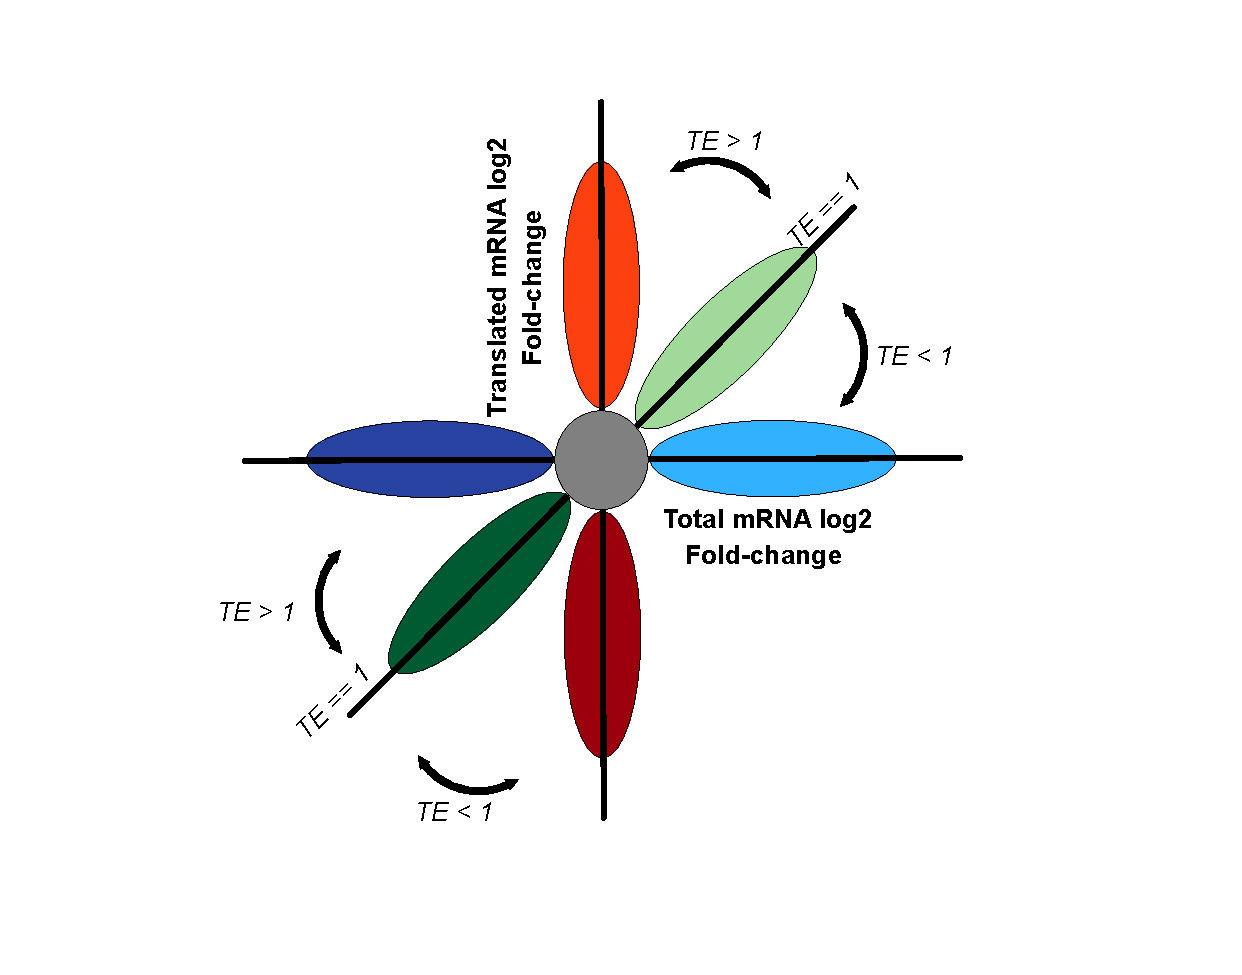
\includegraphics{./figures/geneModes_TE.pdf}
  \caption{TE scores for regulatory modes of gene expression -  Schematic representation of regulatory modes of translation efficiency in a fold-change scatter plot. Indicated in red are changes in translation efficiency altering protein levels, in green changes in mRNA abundance and in blue changes in translation efficiency leading to translational buffering/offsetting. The shifts for the translation efficiency (TE) score are indicated. \label{fig:TE}}
\end{wrapfigure}

\textbf{Figure \ref{fig:TE}} gives an overview of the relationship
between a change in TE and each regulatory mode of gene expression
(\textbf{see also figure \ref{fig:modes}}). Changes in mRNA abundance
will lead to a \(\varDelta\)TE close to 0 in log space (i.e.~no change)
as total mRNA and translated mRNA change with a similar magnitude.
However, in the case of both translation and translational buffering,
terms in the TE-score equation change leading to a \(\varDelta\)TE (TE
\textless{} 0 or TE \textgreater{} 0) and thereby identification of both
changes in translation and translational buffering simultaneously.
Therefore, the TE-score method fails to differentiate between changes in
translation and translational buffering which can have drastic
consequences for the biological interpretation of the results (Oertlin
et al., 2019) (\textbf{see also section \ref{modes}}).

The TE-score approach was challenged by the Analysis of Translation
Activity (anota) algorithm which was developed for DNA-microarray data
(Larsson, Sonenberg, \& Nadon, 2011). anota combines analysis of partial
variance (APV)(Schleifer, Eckholdt, Cohen, \& Keller, 1993) with a
random variance model (RVM)(G. W. Wright \& Simon, 2003). RVM estimates
gene variance using shared information across all genes to increase
power for detection of differential expression(G. W. Wright \& Simon,
2003). anota uses a two-step process that firstly assesses the model
assumptions for (i) absence of highly influential data points, (ii)
common slopes of sample classes, (iii) homoscedasticity of residuals and
(iv) normal distribution of per gene residuals. In the second step then
performs analysis of changes in translational activity using the
following model:

\[log(y_{gi}) = \beta_g^{RNA}\ X_i^{RNA}+ \beta_g^{cond}\ X_i^{cond} + \varepsilon_{gi}\]

here \(\beta_g^{RNA}\) described the relationship to total RNA \(gth\)
gene \(ith\) sample of model matrix \(X\); \(\beta_g^{cond}\) represent
the log2 fold change for treatment classes and \(\varepsilon_{gi}\)
denotes the residual error.

\begin{wrapfigure}{o}{0.5\textwidth}
  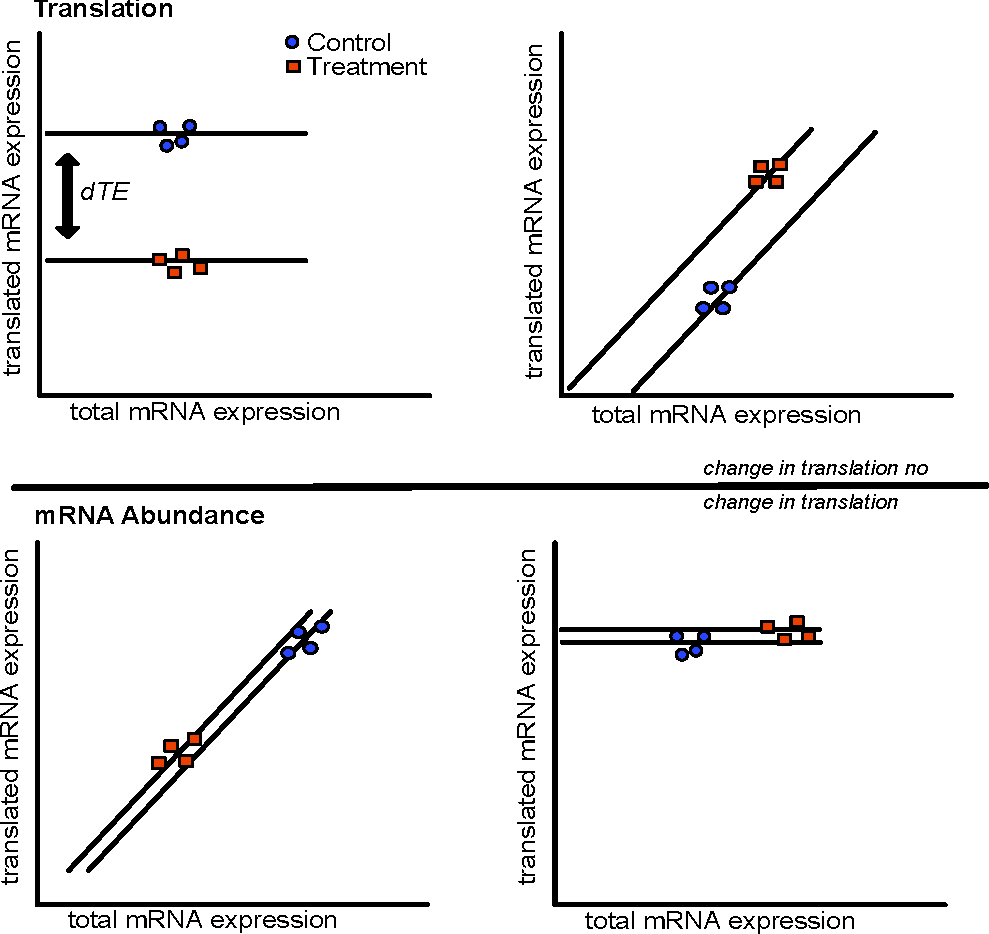
\includegraphics{./figures/geneModes_anota_Larsson.pdf}
  \caption{anota gene models - Schematic representation of the anota analysis models. Translation mRNA expression is set out against total mRNA expression for each biological replicate and treatment condition. Top left shows the model of a gene that is differentially translated (i.e. change in translated but not total mRNA). The difference in the slope intercepts are used to estimate changes in translation efficiencies between conditions i.e. dTE. Other gene models are shown; change in translation efficiency with varying total mRNA levels (top right); change in mRNA abundance (bottom left) and translational buffering (bottom right).
  \label{fig:anota}}
\end{wrapfigure}

Within anota a common slope for the treatment classes that describes the
translated mRNA to total mRNA relationship is calculated. The difference
between the slope intercepts is then interpreted as the \(\varDelta\)
TE. A simplified view of this model can be seen in (\textbf{Figure
\ref{fig:anota} top left}). Here expression for translated mRNA and
total mRNA are modeled over two sample classes with each 4 replicates.
Furthermore, changes in translation efficiencies can also be observed
when translated mRNAs shift to a larger extent than the total mRNA
levels (\textbf{Figure \ref{fig:anota} top right}). Identification of
genes in this categorie can be a challenge, especially in highyl
variable data set, as they resemble mRNA abundance genes (\textbf{Figure
\ref{fig:anota} bottom left}). Nevertheless, Using the linear regression
analysis anota accurately corrects changes in translated mRNA as can be
seen in (\textbf{Figure \ref{fig:anota} bottom right}) where a change in
total mRNA but not translated mRNA levels is observed. For this gene the
difference in slope intercepts is small and will not be identified as
difference in translation as would be the case in the TE-score approach.
anota was developed at a time where translational buffering was
uncommonly seen in data sets. Naturally, the methods lacks a setting to
analyse translational buffering. This was addressed in anota's
successor, anota2seq, and will be discussed in \textbf{Study 1}.

Advances in experimental methods warrant for appropriate statistical
methods to analyse data resulting from them. DNA- microarray was the
dominant platform to assess genome-wide changes before the advent of RNA
sequencing. In DNA- microarray RNA hybridizes probes on a chip and
generate a signal of which the measured intensity is an indicator of
expression, whereas in RNA sequencing reads from RNAs are counted.
Intensity data from DNA microarray can be normalised and transformed
(i.e.~log transformation) to fulfill the requirements for application of
linear models, whereas RNA sequencing harbours additional
characteristics that need to be accounted for. Therefore, algorithms
developed for analysis of DNA- microarray are not directly applicable to
RNA sequencing data as is the case for the anota algorithm.

RNA sequencing data shows variance that is greater than the mean which
is commonly referred to as overdispersion. Count data from RNA
sequencing have been initially approached using Poisson distributions
which assumes that the variance is equal to the mean(J. Lu et al.,
2005). Now established RNA sequencing analysis frameworks such as edgeR
and DESeq2 use negative binomial distributions in combination with
generalized linear models (GLMs) (Robinson, McCarthy, \& Smyth, 2010,
Love, Huber, \& Anders (2014)). The negative binomial distribution uses
a dispersion parameter to account for differences in the mean-variance
relationship across the expression range (McCarthy, Chen, \& Smyth,
2012). While analysis principles of DESeq2 and edgeR are similar they
differ in their normalisation method, dispersion estimation and
information sharing across genes. In a simple differential expression
analysis between two conditions with one RNA type the GLM model would be
as in the following equation:

\[log(y_{gi}) = \beta_g^{cond}\ X_i^{cond} + \varepsilon_{gi}\]

here \(\beta_g^{cond}\ X_i^{cond}\) represent the condition
(i.e.~control and treatment) log2 fold change for the \(gth\) gene
\(ith\) sample of the model matrix X and \(\varepsilon_{gi}\) denotes
the residual error. When analysing changes in translation effiencies
additional parameter for RNA type (i.e.~total mRNA or translated mRNA)
and the interaction between the RNA type and condition are added so
that:

\[log(y_{gi}) = \beta_g^{RNA}\ X_i^{RNA}+ \beta_g^{cond}\ X_i^{cond} + \beta_g^{RNA:cond}\ X_i^{interaction} + \varepsilon_gi\]

In this model the interaction term is interpreted as the change in
translation effiencies (Chothani et al., 2019). Other methods
(i.e.~Ribodiff(Zhong et al., 2017), Riborex(W. Li, Wang, Uren, Penalva,
\& Smith, 2017) and deltaTE (Chothani et al., 2019)) borrow this
analysis principle of an GLM with an interaction term by often applying
this exact model. A noteable difference is that Ribodiff allows
dispersion estimation for translated mRNA and total mRNA separetly as
variance differences between the RNA types can be expected due to
varying experimental protocols (Zhong et al., 2017, Liang et al.
(2018)). While the flexibility of GLMs allows for complex study designs
involving 2 or more treatment conditions, Riborex and Ribodiff limit the
study design to only two conditions. DeltaTE gives their users full
flexibility of the DESeq2 GLM model. Xtail is a method developed for
ribosome profiling that makes use of DESeq2 for RNAseq count
normalisation (Z. Xiao, Zou, Liu, \& Yang, 2016). Their assessment of
differences in translation efficiencies relies on probability matrices
for the ratio of translated mRNA over total mRNA within condition and a
between condition ratio of these ratios. Babel was the first algorithm
designed solely for analysis of differential translation and uses an
error-in-varaibles regression analysis (A. B. Olshen et al., 2013). The
error-in- variables regression allows accounting for variable total mRNA
levels when assessing changes in translation. Although these methods
have distinct approaches to identify changes in translation
efficiencies, their principle of analysis is similar to comparing a
ratio of ratios. Therefore these methods suffer from similar issues as
the TE-score which will be discussed in \textbf{Study 1}.

\chapter{Aims of this thesis}

The aims of this thesis are to expand current methodologies for analysis
of translation efficiency data and explore the regulation of gene
expression in cancer.

In \textbf{Study I} we adapted an algorithm for ANalysis Of Translation
Activity data (anota) so that it could be applied to next generation
sequencing data. Furthermore, we implemented the analysis of
translational buffering a recently described regulatory mode of gene
expression. The resulting algorithm was named anota2seq.

We then applied the anota2seq algorithm to investigate changes in
translation efficiencies in two cancer models:

In \textbf{Study II} we unravelled the effects of eIF4A, an RNA
helicase, inhibition using a synthetic rocaglate CR-1-31-B (CR-31) in
pancreatic ductal adenocarcinoma.

In \textbf{Study III} we explored the effects of insulin on gene
expression in multiple cell lines.

\chapter{Results and discussion}

\section{Study 1 - Generally applicable transcriptome-wide analysis of translation using anota2seq}

Initially changes in translation efficiencies were estimated using the
TE-score approach as outlined in section \ref{algorithm}. However, this
method was being shown to be prone to identification of spurious
correlations leading to elevated false positive identification that can
result in false biological conclusions (Larsson et al., 2010). The
identification of spurious correlations, when using the TE-score, can be
attributed the inadequate correction for changes in total mRNA levels
when estimating translation efficiencies (Larsson et al., 2010,Larsson
et al. (2011)). The Analysis of Translation Activity (anota) algorithm
facilitates analysis of translational efficiencies that are corrected
for changes in total mRNA levels and therefore is not prone to spurious
correlations(Larsson et al., 2011).

anota was developed for analysis of transcriptome-wide analysis for data
quantified by DNA- microarrays (Larsson et al., 2010). However, advances
in experimental methodologies lead to the development in RNA sequencing.
RNA sequencing and DNA microarray data have distinct characteristics
that need to be accounted for before analysis (\textbf{see section
\ref{algorithm}}). Therefore, while the statistical framework of anota
had been shown as an adequate approach for analysis of translational
efficiencies for data from DNA microarrays it was not directly
applicable to RNA sequencing data. The characteristic of RNA sequencing
data, that makes applying anota directly not possible, is the mean
variance relationship. This encompasses that the counts for lower
expressed genes show higher variability than counts for higher expressed
genes even after log transformation. Efforts have been made to make RNA
sequencing data more DNA- microarray like so that algorithms developed
for intensity based microarray data can be applied to count based RNA
sequencing data (Law, Chen, Shi, \& Smyth, 2014,Love et al. (2014)).
Anota2seq, the algorithm developed in this study, allows for
transformation and normalisation of RNA sequencing data so that the
anota statistical frame work can be applied for analysis of count data.

Another feature of anota2seq is that it allows for statistical analysis
of translational buffering. The need for the analysis of translational
buffering, or the uncoupling of transcription from translation, has been
noted before anota2seq's development by comparing 20 translatomes and
transcriptomes with different underlying stimuli in mammalian cells
(Tebaldi et al., 2012). The same authors proposed a framework, called
tRanslatome, that combines several methodologies for analysis of
differential transcription and translation efficiencies, including
anota, for a comprehensive analysis of transcription and translation as
well as their underlying mechanisms (Tebaldi, Dassi, Kostoska, Viero, \&
Quattrone, 2014).

\begin{wrapfigure}{o}{0.5\textwidth}
  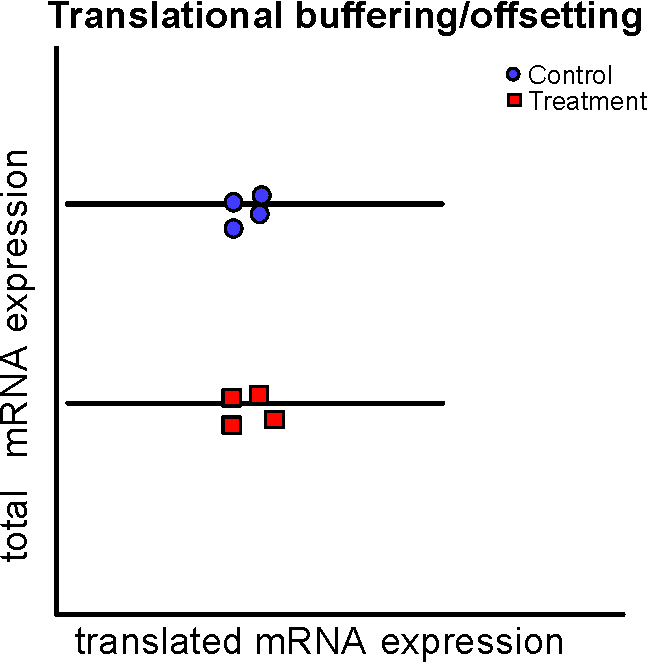
\includegraphics{./figures/geneModes_anota2seq.pdf}
  \caption{anota2seq gene model for analysis of translational buffering /offsetting - Total mRNA expression is set out against translated mRNA expression for each biological replicate and treatment condition. The model shows total mRNA changes that are independent of translated mRNA changes which is classified as translational buffering. It is important to distinguish between the gene modes as their regulation could be due to different underlying biological mechanisms (see section \ref{modes}).
  \label{fig:anota2seq}}
\end{wrapfigure}

Nevertheless, commonly observed in polysome and ribosome profiling data
sets are three gene expression modes, translation, translational
buffering and mRNA abundance. While anota can be used to identify genes
among the translation and mRNA abundance mode, analysis for
translational buffering was not implemented therein (\emph{See Figure
\ref{fig:anota}}). Therefore, one would need to rely on the integration
of several methods to efficiently analyse transcriptome-wide studies of
translation efficiences. Anota2seq addresses this issue by changing the
analysis model as described in section \ref{algorithm} to analyse
changes in total mRNA levels corrected for changes in translated mRNA
levels (i.e.~translational buffering, \textbf{see figure
\ref{fig:anota2seq}}).

Appliance of anota2seq has successfuly identified translational
buffering to which biological mechanisms could be linked,e.g.~as
mentioned earlier translationally bufferring under ER\(\alpha\)
depletion in prostate cancer (\textbf{see section \ref{modeBuffering}})
(Lorent et al., 2019). Furthermore, in \textbf{study 2} translational
buffering can be observed as a compensating mechanisms in ``healthy''
cells upon treatment with an eIF4A inhibitor and in \textbf{study 3} we
identify mTOR dependent translational buffering for mRNAs with certain
3' UTR charactersitics.

The aim of this study is to compare anota2seq's performance to other
established algorithms (i.e.~DESeq2, RiboDiff, babel, TE-score and
Xtail) for analysis of translation efficiencies, specifically their
ability to distinguish the three prominent modes of gene expression. To
achieve we used a simulated data based approach. While it is arguable to
what extent conclusion drawn from simulated data can be extended towards
empircal data it allows for a controlled environment where true positive
changes are known in advance. Furthermore, the mean-variance
relationship in the simulated data is based on a real polysome profiling
data set to increase confidence that drawn conclusions are also
applicable to emprical data (Guan et al., 2017).

The simulated data consisted of four replicates for translated mRNA and
total mRNA with a ``control'' and a ``treatment'' condition.
Furthermore, the data sets contained a combination of the following gene
sets:

``Unchanged'': For this simulation category we drew reads from the same
NB distrubution for both the control and treatment conditions in both
the translated and total mRNA. This catergory reprents genes that would
be unaffected by e.g.~a stimulus of between cellular states.

``mRNA abundance'': For this category the control condition for both the
translated mRNA and total mRNA were drawn from the same NB distribution.
The NB distribution for \emph{both translated mRNA and total mRNA} of
the treatment condition was altered so that values would be drawn
corresponding to a fold change (negative or positive) ranging between
1.5 to 3.0. The directionality of the fold changes (i.e.~up or down
regulation) was the same for translated mRNA and total mRNA.

``translation'': For this category the control condition for both the
translated mRNA and total mRNA were drawn from the same NB distribution.
The NB distribution for \emph{translated mRNA only} of the treatment
condition was altered so that values would be drawn corresponding to a
fold change (negative or positive) ranging between 1.5 to 3.0.

``buffering'': For this category the control condition for both the
translated mRNA and total mRNA were drawn from the same NB distribution.
The NB distribution for \emph{total mRNA only} of the treatment
condition was altered so that values would be drawn corresponding to a
fold change (negative or positive) ranging between 1.5 to 3.0.

As a first step we tested whether the methods could properly control for
type-1 errors (i.e.~false positive identifcation). For this we simulated
a data set with genes belonging only to the ``unchanged'' category. This
revealed that babel, but to an even greater extent Xtail, were unable to
control their type-1 error as these methods assigned low p-values and
FDRs when no real changes were present. This indicated a limited
applicability of Xtail and babel for statistical analysis of
translatomes.

From the comparative analysis of the analysis for changes in translation
efficiencies affecting protein levels we concluded that anota2seq
outperforms all other methods. This was assessed by comparing the area
under the curve from Receiver operating characteristics (ROC) and
precision recall curves. The ROC curves showed a, albeit slightly,
better performance for detecting changes in translation. However, the
precision recall was much higher for anota2seq which can be accredited
to that the analysis principle of the other methods is based on
identifying changes regardless of whether the change is in the
translated mRNA or total mRNA (\emph{as explained in section
\ref{algorithm}}). Nevertheless, when comparing the performance using
simulatd data in the absence of genes belonging to the ``buffering''
category anota2seq still showed superior performance.

Next to the a prior knowledge of the introduced changes in the
simulation data, it also allowed us to modify parameters to investigate
the robustness of the methods to increased variance, overall sequencing
depth and differing sequencing depth between samples. Here, all methods
showed robustness against variance and sequencing depth differences
between samples as long as a minimum of 5 million counts per sample was
reached.

A short coming in the simulation study is that we did not assess the
effects of systematic batch effects. Batch effects can be introduced
e.g.~during experimental design and there are many methods that try to
correct for these(W. E. Johnson, Li, \& Rabinovic, 2007,Leek (2014),Y.
Zhang, Parmigiani, \& Johnson (2020)). Other ways to correct for batch
effects is their inclusion in the analysis model, which can be supplied
to the analysis model in DESeq2, edgeR as well as anota2seq. Indeed
analysis of a dataset with prominent batch effects showed that batch
effects can dampen the efficiency of the anota2seq algorithm to identify
changes but can be effectively corrected for in the algorithm.

In this study we developed an analysis algorithm for efficient
transcriptome-wide analysis of translation efficiencies applicable to
DNA-microarrays and RNA seq. Furthermore, anota2seq has been
successfully applied to broaden the knowledge around mRNA translation in
various different contexts (Lorent et al., 2019,Chan et al.
(2019),Hipolito et al. (2019),Chaparro et al. (2020)).

\section{Study 2 - eIF4A supports an oncogenic translation program in pancreatic ductal adenocarcinoma}

Pancreatic cancer is considered a lethal malignancy and has limitited
treatment options. A study on predicitons for european cancer mortality
rates for 2021 concluded that health efforts should focus on pancreatic
cancer. While other cancers (e.g.~ovary, breast and stomach) showed a
decline in mortality rates, no major overall decline was observed for
pancreatic cancer in the period of 1970-2021 (Carioli et al., 2021).

Pancreatic ductal adeno carcinoma (PDAC) accounts for over 90\% of
exocrine pancreatic cancer, whereas non ductal pancreatic cancers
e.g.~acinar cell carcinomas are uncommon (Feldmann, Beaty, Hruban, \&
Maitra, 2007,Jun \& Hong (2016)). It is estimated the 60-70\% of the
PDACs arise in the head (Luchini, Capelli, \& Scarpa, 2016). So far
treatment options are mostly limited to surgical removal, which can be
complicated due to the anatomical location of the pancreas head.

With the increasing understanding of tumor heterogeneity, i.e.~tumors
with similar tissue origin are not necessarily identical at a molecular
level, anti cancer therapy improved (Biankin \& Hudson, 2011). In breast
cancer stratification by histological,molecular and gene expression
features lead to identification of several breast cancer subtypes for
which different treatment options exist, e.g. \(ER^+\) breast cancer
subtypes respond to endocrine therapy whereas \(ER^-\) do not(Andre \&
Pusztai, 2006,Parker et al. (2009)). While breast canacer treatment
strategies benefit from a rather well established understanding of the
molecular subtypes, in pancreatic cancer trascriptomic based subtyping
is still ongoing (P. Bailey et al., 2016,Puleo et al. (2018),Collisson
et al. (2011),Moffitt et al. (2015),Collisson, Bailey, Chang, \& Biankin
(2019)). Therefore, it is warranted to extend current knowledge around
pancreatic cancer to advance therapeutic strategies in this lethal
disease.

Nevertheless, commonly shared among PDAs are oncogenic mutations in KRAS
as well as inactivation of tumor supressors e.g.~TP53 (S. Jones et al.,
2008). Furthermore, PDAs have been shown to be dependent on increased
protein synthesis mediated by Kras (Chio et al., 2016). This indicates
an important role of mRNA translation in PDA.

The aim of \emph{study 2} was to investigate the therapeutic effects of
targetting eIF4A in a three dimensional PDA organoid cell culture with
mutations in the \(Kras^{LSL-G12D}\), \(Trp53^{LSL-R172H}\) and Pdx1-cre
alleles that has been shown to recapitulate PDA tumor progression (Boj
et al., 2015). The inhibition of eIF4A was done using a synthetic
rocaglate, CR-1-31B (CR-31). Rocaglates have been shown to inhibit eIF4A
helicase activity and displayed anti tumor activity (Cencic et al.,
2009).

We first wanted to establish the therapeutic validity of targetting
eIF4A in PDA. In vitro experiments comparing treated PDA organoids (KP)
to their normal (N) counter parts revealed hightened sensitivity of PDA
organoids to CR-31 treatment. OP-puromycin incorporation showed reduced
protein synthesis in KP, whereas N were affected to a lesser extent.
Furthermore, similar effects were found in vivo for PDA tumours where
also CR-31 reduced protein synthesis (assessed by SUnSET assay), tumor
growth (assessed by ultra sound imaging) and increased survival. The
effect on protein synthesis was not due to inhibition of oncogenic
signalling pathways which was evaluated western blot assessing the
phosphorylation of e.g.~AKT, mTOR and 4E-BP1. From these findings we
concluded that there is therapeutic validity in targetting eIF4A in PDA
that acts downsteam of oncogenic signalling pathways.

Using polysome profiling we then sought to decipher the mechanisms
explaining the increased sensivity to CR-31 in KP organoids. First we
investigated the differences in gene expression between untreated KP and
N organoids. Analysis of changes in translation efficiencies using
anota2seq revealed massive modulation at both transcription and
translation indicative of the underlying differences in e.g.~genomic
stability and enhanced oncogenic signalling impinging on protein
synthesis. Consistent with the in vitro OP-puromycin incorporation and
in vivo SUNsET experiments, CR-31 had only little effect on translation
in N organoids, whereas in KP organoids exclusively changes in
translation were detected.

We then compared the mRNAs affected by CR-31 in KP to the acquired
translational profile of untreated KP and N organoids. In order to
achieve this we visualised the mRNAs affected by CR-31 in KP onto the
data of the untreated KP vs N organoids comparison. This revealed that
the acquired translational program of KP organoids is reversed when
treated with CR-31.

Performing a similar analysis, we visualised mRNAs sensitive to CR-31 in
KP onto the data of the CR-31 treated N organoids. mRNAs affected by
CR-31 in KP were translationally buffered in CR-31 treated N organoids.
Translational buffering, as an adaptive response to treatment, has been
shown to maintain protein homeostasis by inducing a transcriptional
response increasing the pool of mRNAs that can be translated (Lorent et
al., 2019). The ability for N organoids in increase transcription for
mRNAs affected by CR-31, whereas KP cannot, could partially explain as
to why protein synthesis is not reduced to a similar extent in N as in
KP.

We then assessed 5' UTR characteristics of the translationally regulated
mRNAs upon CR-31 treatment in KP organoids. It was reported that
eIF4A-senstive mRNAs showed overall and more structured 5' UTRs
(e.g.~containing G-quadruplexes) (Rubio et al., 2014,Wolfe et al.
(2014),Gandin et al. (2016b)). Furthermore, a mechanisms by which
rocaglates would clamp eIF4A to mRNAs with {[}A,G{]} repeats in their 5
UTR was described (Iwasaki, Floor, \& Ingolia, 2016). However, mRNAs
sensitive to CR-31 treatment herien showed overall shorter 5' UTRs that
were more structured when corrected for their length without enrichment
for 4G-quadruplexes or {[}A,G{]} repeats. From the polysome profiling
and UTR analysis we concluded that eIF4A supports an oncogenic
translation program in PDA cells for mRNAs with shorter but structured
5' UTRs.

Shorter 5' UTRs have been shown to be sensitive to eIF4E expression and
enconde for metabolic functions (see section \ref{regmRNA}). When we
compared an eIF4E overexpression signature in the KP vs N and CR-31
treated KP we observed that in KP organoids translationally regulated
mRNAs under eIF4E overexpression were also translationally activated.
This observation is consistent with reports of 4E-BP1 loss in pancreatic
cancer (Y. Martineau et al., 2014). CR-31 treatment in KP reversed the
translational profile for these mRNAs. Therefore, while rocaglates have
been shown to directly target eIF4A (Cencic et al., 2009). eIF4A
inhibition in tumors resistant to mTOR inhibiton by loss of 4E-BP1 has
been shown to circumvent this resistance (D. Müller et al., 2019).
Therefore, eIF4F complex formation could be disrupted by reduced eIF4A
availability to an extent that also cap dependent translation is
affected in PDA organoids herein.

When further inspecting the regulated gene sets in treated and untreated
KP compared to their normal counterparts we could see an enrichtment in
metabolic pathways, e.g.~Oxidative phosphorylation. This pathway was
upregulated in untreated KP compared to N, whereas in KP CR-31 treatment
reversed the translational profile of this pathway. These findings were
experimentally validated and shown to disrupt the mitochondrial
respiration (measured by oxygen consumption rates).

A way to counter loss of energy production through oxidative
phosphorylation is to increase activity of other anaerobic metabolic
pathways, i.e.~glycolysis. However, in CR-31 treated KP we could not
detect a upregulation of glycolysis measured by \(U-C^{13}\) glucose
labeling and extra cellular acidification rates nor did CR-31 treatement
affect expression of glycolytic enzymes (e.g.~HK1,HK2, LDHA, SLCA1,
SLCA3). Furthermore, glucose deprivation did not further sensitise to
CR-31 treatment. This was rather unexpected, given that increased
glycolysis is characteristic for cancers as described by Otto walburg
(Warburg, Wind, \& Negelein, 1927). However, the polysome prolfing data
revealed translational downregulation and subsequent reduction of
protein expression for the glucose transporter Slc2a6. Indeed,
perturbation of Slc2a6 using \(sgRNA^{Slc2a6}\) in N and KP organoids
revealed a decrease in glucose uptake. From this we concluded that
glycolytic compensation of KP is diminished by translational regulation
of the glucose transporter Slc2a6 upon CR-31 treatment.

Among the translationally activated genes in the CR-31 treated KP
organoids where mRNAs involved in the glutamine metabolism (i.e.~Slc1a5
and Gls1). Furthermore, glutamine levels were elevated in patient
derived PDA cell lines treated with CR-31. Glutamine can be converted
into \(\alpha\)-ketoglutarate and funneled into the krebs cycle and
therefore can serve to increase energy production (D. Xiao et al.,
2016). Indeed, using gas chromatography mass spectrometry (GC/MS) to
quantify downstream metabolites after culturing PDA cells in
\(C_5^{13}\)- glutamine, we identified a shift towards reductive
carboxylation of \(\alpha\)-ketoglutarate obtained from \(C_5^{13}\)-
glutamine to produce acetyl-CoA. Notably, the glutamine metabolism was
not elevated in N organoids.

A combined treatment of CR-31 with glutaminase inhibitors (BPTES or
CB839) could sensitise to CR-31 treatment patient-derived PDA cells to
CR-31 treatment. Therefore, our study suggests an eIF4A dependent
translational program in PDA that can act as a theurapeutic target in
PDA. Furthermore, a recently published ribosome profiling study of a
CR-31 treated human pancreatic cancer cell line (PANC1) observed the
same therapeutic effect of CR-31 treatment in vivo on survival and tumor
volume (Singh et al., 2021). This underlines the significance of our
study in identifying eIF4A as therapeutic target in PDA.

Nevertheless, the same study indicated differences on the underlying
regulated mRNA subsets. They report, in line with the literature, that
eIF4A depdent mRNAs show long and structured 5' UTRs containing
G-quadruplexes (Singh et al., 2021,Wolfe et al. (2014)). While the 5'
UTRs of the mRNAs identified herein where overall shorter, they were
overall more structured. Furthermore, the mRNAs identifed in Singh et.
al. were involved in KRAS signalling, which was unaltered in our study.

This raises some questions about the differences between experimental
setups and their potential influence on biological outcomes. For
instance, Singh et. al. performed ribosome profiling on a PANC1 cell
line culture treated with 25nM CR-31, wheres herein we performed
polysome profiling on a 3D-organoid culture treated with 10nM CR-31. The
differences between ribosome and polysome profiling have been discussed
extensively (see section \ref{exptMethod}). However, by measuring IC50
concentrations for CR-31 in a panel of pancreatic cancer cell lines, the
autors show a \textasciitilde{}6-fold difference in susceptability to
CR-31. PANC1 cells were most affected by CR-31. Dosage dependent
viability experiments of patient derived PDA cells in our study revealed
that at 10nM viability was reduced by \textasciitilde{}30\%, whereas
treatment with 25nM reduced viability by \textgreater{} 50\%.
Furthermore, a combination treatment of CR-31 and CB839 showed no
difference at 25nM CR-31, whereas at 12.50nM a difference was observed.
Therefore, combining the findings of these two studies indicate that
CR-31 treatment in PDA indeed has a therapetuic effect, however the
underlying mechanisms that are observed in the transcriptome wide
analysis of translation efficiencies are likeley dependent on the cell
culture and treatment dosages.

\section{Study 3 - mTOR-dependent translational buffering overrides transcriptome alterations leading to
maintained proteome composition}

\chapter{Conclusions}

\chapter*{Acknowledgments}\label{acknowledgments}
\addcontentsline{toc}{chapter}{Acknowledgments}

\chapter*{References}\label{references}
\addcontentsline{toc}{chapter}{References}

\hypertarget{refs}{}
\hypertarget{ref-Afonina2014}{}
Afonina, Z. A., Myasnikov, A. G., Shirokov, V. A., Klaholz, B. P., \&
Spirin, A. S. (2014). Formation of circular polyribosomes on eukaryotic
mRNA without cap-structure and poly(A)-tail: A cryo electron tomography
study. \emph{Nucleic Acids Research}, \emph{42}(14), 9461--9469.
\url{https://doi.org/10.1093/nar/gku599}

\hypertarget{ref-Alkalaeva2006}{}
Alkalaeva, E. Z., Pisarev, A. V., Frolova, L. Y., Kisselev, L. L., \&
Pestova, T. V. (2006). In Vitro Reconstitution of Eukaryotic Translation
Reveals Cooperativity between Release Factors eRF1 and eRF3.
\emph{Cell}, \emph{125}(6), 1125--1136.
\url{https://doi.org/10.1016/j.cell.2006.04.035}

\hypertarget{ref-Amrani2008}{}
Amrani, N., Ghosh, S., Mangus, D. A., \& Jacobson, A. (2008).
Translation factors promote the formation of two states of the
closed-loop mRNP. \emph{Nature}, \emph{453}(7199), 1276--1280.
\url{https://doi.org/10.1038/nature06974}

\hypertarget{ref-Andre2006}{}
Andre, F., \& Pusztai, L. (2006). Molecular classification of breast
cancer: Implications for selection of adjuvant chemotherapy.
\emph{Nature Clinical Practice Oncology}, \emph{3}(11), 621--632.
\url{https://doi.org/10.1038/ncponc0636}

\hypertarget{ref-Andreev2015}{}
Andreev, D. E., O'Connor, P. B., Fahey, C., Kenny, E. M., Terenin, I.
M., Dmitriev, S. E., \ldots{} Baranov, P. V. (2015). Translation of
5\({'}\) leaders is pervasive in genes resistant to eIF2 repression.
\emph{ELife}, \emph{4}, e03971.
\url{https://doi.org/10.7554/eLife.03971}

\hypertarget{ref-Artieri2014}{}
Artieri, C. G., \& Fraser, H. B. (2014). Evolution at two levels of gene
expression in yeast. \emph{Genome Research}, \emph{24}(3), 411--421.
\url{https://doi.org/10.1101/gr.165522.113}

\hypertarget{ref-Asano2000}{}
Asano, K., Clayton, J., Shalev, A., \& Hinnebusch, A. G. (2000). A
multifactor complex of eukaryotic initiation factors, eIF1, eIF2, eIF3,
eIF5, and initiator tRNAMet is an important translation initiation
intermediate in vivo. \emph{Genes \& Development}, \emph{14}(19),
2534--2546. \url{https://doi.org/10.1101/gad.831800}

\hypertarget{ref-Bailey2016}{}
Bailey, P., Chang, D. K., Nones, K., Johns, A. L., Patch, A.-M.,
Gingras, M.-C., \ldots{} Grimmond, S. M. (2016). Genomic analyses
identify molecular subtypes of pancreatic cancer. \emph{Nature},
\emph{531}(7592), 47--52. \url{https://doi.org/10.1038/nature16965}

\hypertarget{ref-Baou2011}{}
Baou, M., Norton, J. D., \& Murphy, J. J. (2011). AU-rich RNA binding
proteins in hematopoiesis and leukemogenesis. \emph{Blood},
\emph{118}(22), 5732--5740.
\url{https://doi.org/10.1182/blood-2011-07-347237}

\hypertarget{ref-Bhat2015}{}
Bhat, M., Robichaud, N., Hulea, L., Sonenberg, N., Pelletier, J., \&
Topisirovic, I. (2015). Targeting the translation machinery in cancer.
\emph{Nature Reviews Drug Discovery}, \emph{14}(4), 261--278.
\url{https://doi.org/10.1038/nrd4505}

\hypertarget{ref-Biankin2011}{}
Biankin, A. V., \& Hudson, T. J. (2011). Somatic variation and cancer:
Therapies lost in the mix. \emph{Human Genetics}, \emph{130}(1), 79--91.
\url{https://doi.org/10.1007/s00439-011-1010-0}

\hypertarget{ref-Boj2015}{}
Boj, S. F., Hwang, C.-I., Baker, L. A., Chio, I. I. C., Engle, D. D.,
Corbo, V., \ldots{} Tuveson, D. A. (2015). Organoid Models of Human and
Mouse Ductal Pancreatic Cancer. \emph{Cell}, \emph{160}(1), 324--338.
\url{https://doi.org/10.1016/j.cell.2014.12.021}

\hypertarget{ref-Brar2015}{}
Brar, G. A., \& Weissman, J. S. (2015). Ribosome profiling reveals the
what, when, where and how of protein synthesis. \emph{Nature Reviews.
Molecular Cell Biology}, \emph{16}(11), 651--664.
\url{https://doi.org/10.1038/nrm4069}

\hypertarget{ref-Buttgereit1995}{}
Buttgereit, F., \& Brand, M. D. (1995). A hierarchy of ATP-consuming
processes in mammalian cells. \emph{The Biochemical Journal}, \emph{312
( Pt 1)}(Pt 1), 163--7. \url{https://doi.org/10.1042/bj3120163}

\hypertarget{ref-Calvo2009}{}
Calvo, S. E., Pagliarini, D. J., \& Mootha, V. K. (2009). Upstream open
reading frames cause widespread reduction of protein expression and are
polymorphic among humans. \emph{Proceedings of the National Academy of
Sciences}, \emph{106}(18), 7507--7512.
\url{https://doi.org/10.1073/pnas.0810916106}

\hypertarget{ref-Carioli2021}{}
Carioli, G., Malvezzi, M., Bertuccio, P., Boffetta, P., Levi, F.,
Vecchia, C. L., \& Negri, E. (2021). European cancer mortality
predictions for the year 2021 with focus on pancreatic and female lung
cancer. \emph{Annals of Oncology}, \emph{0}(0).
\url{https://doi.org/10.1016/j.annonc.2021.01.006}

\hypertarget{ref-Cencic2009}{}
Cencic, R., Carrier, M., Galicia-Vázquez, G., Bordeleau, M.-E.,
Sukarieh, R., Bourdeau, A., \ldots{} Pelletier, J. (2009). Antitumor
Activity and Mechanism of Action of the Cyclopenta{[}b{]}Benzofuran,
Silvestrol. \emph{PLoS ONE}, \emph{4}(4).
\url{https://doi.org/10.1371/journal.pone.0005223}

\hypertarget{ref-Cenik2015}{}
Cenik, C., Cenik, E. S., Byeon, G. W., Grubert, F., Candille, S. I.,
Spacek, D., \ldots{} Snyder, M. P. (2015). Integrative analysis of RNA,
translation, and protein levels reveals distinct regulatory variation
across humans. \emph{Genome Research}, \emph{25}(11), 1610--1621.
\url{https://doi.org/10.1101/gr.193342.115}

\hypertarget{ref-Chan2019}{}
Chan, K., Robert, F., Oertlin, C., Kapeller-Libermann, D., Avizonis, D.,
Gutierrez, J., \ldots{} Chio, I. I. C. (2019). eIF4A supports an
oncogenic translation program in pancreatic ductal adenocarcinoma.
\emph{Nature Communications}, \emph{10}(1), 5151.
\url{https://doi.org/10.1038/s41467-019-13086-5}

\hypertarget{ref-Chaparro2020}{}
Chaparro, V., Leroux, L.-P., Masvidal, L., Lorent, J., Graber, T. E.,
Zimmermann, A., \ldots{} Jaramillo, M. (2020). Translational profiling
of macrophages infected with Leishmania donovani identifies mTOR- and
eIF4A-sensitive immune-related transcripts. \emph{PLOS Pathogens},
\emph{16}(6), e1008291.
\url{https://doi.org/10.1371/journal.ppat.1008291}

\hypertarget{ref-Cheng2016}{}
Cheng, Z., Teo, G., Krueger, S., Rock, T. M., Koh, H. W. L., Choi, H.,
\& Vogel, C. (2016). Differential dynamics of the mammalian mRNA and
protein expression response to misfolding stress. \emph{Molecular
Systems Biology}, \emph{12}(1), 855.
\url{https://doi.org/10.15252/msb.20156423}

\hypertarget{ref-Chio2016}{}
Chio, I. I. C., Jafarnejad, S. M., Ponz-Sarvise, M., Park, Y., Rivera,
K., Palm, W., \ldots{} Tuveson, D. A. (2016). NRF2 Promotes Tumor
Maintenance by Modulating mRNA Translation in Pancreatic Cancer.
\emph{Cell}, \emph{166}(4), 963--976.
\url{https://doi.org/10.1016/j.cell.2016.06.056}

\hypertarget{ref-Chothani2019}{}
Chothani, S., Adami, E., Ouyang, J. F., Viswanathan, S., Hubner, N.,
Cook, S. A., \ldots{} Rackham, O. J. L. (2019). deltaTE: Detection of
Translationally Regulated Genes by Integrative Analysis of Ribo-seq and
RNA-seq Data. \emph{Current Protocols in Molecular Biology},
\emph{129}(1), e108. \url{https://doi.org/10.1002/cpmb.108}

\hypertarget{ref-Collisson2019}{}
Collisson, E. A., Bailey, P., Chang, D. K., \& Biankin, A. V. (2019).
Molecular subtypes of pancreatic cancer. \emph{Nature Reviews
Gastroenterology \& Hepatology}, \emph{16}(4), 207--220.
\url{https://doi.org/10.1038/s41575-019-0109-y}

\hypertarget{ref-Collisson2011}{}
Collisson, E. A., Sadanandam, A., Olson, P., Gibb, W. J., Truitt, M.,
Gu, S., \ldots{} Gray, J. W. (2011). Subtypes of pancreatic ductal
adenocarcinoma and their differing responses to therapy. \emph{Nature
Medicine}, \emph{17}(4), 500--503. \url{https://doi.org/10.1038/nm.2344}

\hypertarget{ref-Connolly2006}{}
Connolly, E., Braunstein, S., Formenti, S., \& Schneider, R. J. (2006).
Hypoxia inhibits protein synthesis through a 4E-BP1 and elongation
factor 2 kinase pathway controlled by mTOR and uncoupled in breast
cancer cells. \emph{Molecular and Cellular Biology}, \emph{26}(10),
3955--3965. \url{https://doi.org/10.1128/MCB.26.10.3955-3965.2006}

\hypertarget{ref-Crick1970}{}
Crick, F. (1970). Central Dogma of Molecular Biology. \emph{Nature},
\emph{227}(5258), 561--563. \url{https://doi.org/10.1038/227561a0}

\hypertarget{ref-Crick1966}{}
Crick, F. H. (1966). Codon--Anticodon pairing: The wobble hypothesis.
\emph{Journal of Molecular Biology}, \emph{19}(2), 548--555.
\url{https://doi.org/10.1016/s0022-2836(66)80022-0}

\hypertarget{ref-deSousaAbreu2009}{}
de Sousa Abreu, R., Penalva, L. O., Marcotte, E. M., \& Vogel, C.
(2009). Global signatures of protein and mRNA expression levels.
\emph{Molecular BioSystems}, \emph{5}(12), 1512--1526.
\url{https://doi.org/10.1039/b908315d}

\hypertarget{ref-Delaunay2016}{}
Delaunay, S., Rapino, F., Tharun, L., Zhou, Z., Heukamp, L., Termathe,
M., \ldots{} Close, P. (2016). Elp3 links tRNA modification to
IRES-dependent translation of LEF1 to sustain metastasis in breast
cancer. \emph{Journal of Experimental Medicine}, \emph{213}(11),
2503--2523. \url{https://doi.org/10.1084/jem.20160397}

\hypertarget{ref-Deng2015}{}
Deng, W., Babu, I. R., Su, D., Yin, S., Begley, T. J., \& Dedon, P. C.
(2015). Trm9-Catalyzed tRNA Modifications Regulate Global Protein
Expression by Codon-Biased Translation. \emph{PLOS Genetics},
\emph{11}(12), e1005706.
\url{https://doi.org/10.1371/journal.pgen.1005706}

\hypertarget{ref-Denkert2004}{}
Denkert, C., Weichert, W., Winzer, K.-J., Müller, B.-M., Noske, A.,
Niesporek, S., \ldots{} Hauptmann, S. (2004). Expression of the
ELAV-Like Protein HuR Is Associated with Higher Tumor Grade and
Increased Cyclooxygenase-2 Expression in Human Breast Carcinoma.
\emph{Clinical Cancer Research}, \emph{10}(16), 5580--5586.
\url{https://doi.org/10.1158/1078-0432.CCR-04-0070}

\hypertarget{ref-Dever2012}{}
Dever, T. E., \& Green, R. (2012). The elongation, termination, and
recycling phases of translation in eukaryotes. \emph{Cold Spring Harbor
Perspectives in Biology}, \emph{4}(7), 1--16.
\url{https://doi.org/10.1101/cshperspect.a013706}

\hypertarget{ref-Dorner2006}{}
Dorner, S., Brunelle, J. L., Sharma, D., \& Green, R. (2006). The hybrid
state of tRNA binding is an authentic translation elongation
intermediate. \emph{Nature Structural \& Molecular Biology},
\emph{13}(3), 234--241. \url{https://doi.org/10.1038/nsmb1060}

\hypertarget{ref-Dorrello2006}{}
Dorrello, N. V., Peschiaroli, A., Guardavaccaro, D., Colburn, N. H.,
Sherman, N. E., \& Pagano, M. (2006). S6K1- and ßTRCPPMediated
Degradationn ofPDCD4 Promotes Protein Translationn andCell Growth.
\emph{Science}, \emph{314}(5798), 467--471.
\url{https://doi.org/10.1126/science.1130276}

\hypertarget{ref-ElYacoubi2012}{}
El Yacoubi, B., Bailly, M., \& de Crécy-Lagard, V. (2012). Biosynthesis
and Function of Posttranscriptional Modifications of Transfer RNAs.
\emph{Annual Review of Genetics}, \emph{46}(1), 69--95.
\url{https://doi.org/10.1146/annurev-genet-110711-155641}

\hypertarget{ref-Fan1998}{}
Fan, X. C., \& Steitz, J. A. (1998). Overexpression of HuR, a
nuclearCytoplasmic shuttling protein, increases the in vivo stability of
ARE-containing mRNAs. \emph{The EMBO Journal}, \emph{17}(12),
3448--3460. \url{https://doi.org/10.1093/emboj/17.12.3448}

\hypertarget{ref-Feldmann2007}{}
Feldmann, G., Beaty, R., Hruban, R. H., \& Maitra, A. (2007). Molecular
genetics of pancreatic intraepithelial neoplasia. \emph{Journal of
Hepato-Biliary-Pancreatic Surgery}, \emph{14}(3), 224--232.
\url{https://doi.org/10.1007/s00534-006-1166-5}

\hypertarget{ref-Gandin2016}{}
Gandin, V., Masvidal, L., Cargnello, M., Gyenis, L., McLaughlan, S.,
Cai, Y., \ldots{} Topisirovic, I. (2016a). mTORC1 and CK2 coordinate
ternary and eIF4F complex assembly. \emph{Nature Communications},
\emph{7}(1), 11127. \url{https://doi.org/10.1038/ncomms11127}

\hypertarget{ref-Gandin2016a}{}
Gandin, V., Masvidal, L., Hulea, L., Gravel, S.-P., Cargnello, M.,
McLaughlan, S., \ldots{} Topisirovic, I. (2016b). nanoCAGE reveals 5'
UTR features that define specific modes of translation of functionally
related MTOR-sensitive mRNAs. \emph{Genome Research}, \emph{26}(5),
636--648. \url{https://doi.org/10.1101/gr.197566.115}

\hypertarget{ref-Gandin2014}{}
Gandin, V., Sikström, K., Alain, T., Morita, M., McLaughlan, S.,
Larsson, O., \& Topisirovic, I. (2014). Polysome fractionation and
analysis of mammalian translatomes on a genome-wide scale. \emph{Journal
of Visualized Experiments: JoVE}, (87).
\url{https://doi.org/10.3791/51455}

\hypertarget{ref-Gingold2014}{}
Gingold, H., Tehler, D., Christoffersen, N. R., Nielsen, M. M., Asmar,
F., Kooistra, S. M., \ldots{} Pilpel, Y. (2014). A Dual Program for
Translation Regulation in Cellular Proliferation and Differentiation.
\emph{Cell}, \emph{158}(6), 1281--1292.
\url{https://doi.org/10.1016/j.cell.2014.08.011}

\hypertarget{ref-Gingras1999}{}
Gingras, A.-C., Gygi, S. P., Raught, B., Polakiewicz, R. D., Abraham, R.
T., Hoekstra, M. F., \ldots{} Sonenberg, N. (1999). Regulation of 4E-BP1
phosphorylation: A novel two-step mechanism. \emph{Genes \&
Development}, \emph{13}(11), 1422--1437.

\hypertarget{ref-Goodenbour2006}{}
Goodenbour, J. M., \& Pan, T. (2006). Diversity of tRNA genes in
eukaryotes. \emph{Nucleic Acids Research}, \emph{34}(21), 6137--6146.
\url{https://doi.org/10.1093/nar/gkl725}

\hypertarget{ref-Goke2002}{}
Göke, A., Göke, R., Knolle, A., Trusheim, H., Schmidt, H., Wilmen, A.,
\ldots{} Chen, Y. H. (2002). DUG is a novel homologue of translation
initiation factor 4G that binds eIF4A. \emph{Biochemical and Biophysical
Research Communications}, \emph{297}(1), 78--82.
\url{https://doi.org/10.1016/S0006-291X(02)02129-0}

\hypertarget{ref-Graff2009}{}
Graff, J. R., Konicek, B. W., Lynch, R. L., Dumstorf, C. A., Dowless, M.
S., McNulty, A. M., \ldots{} Carter, J. H. (2009). eIF4E activation is
commonly elevated in advanced human prostate cancers and significantly
related to reduced patient survival. \emph{Cancer Research},
\emph{69}(9), 3866--3873.
\url{https://doi.org/10.1158/0008-5472.CAN-08-3472}

\hypertarget{ref-Grifo1983}{}
Grifo, J. A., Tahara, S. M., Morgan, M. A., Shatkin, A. J., \& Merrick,
W. C. (1983). New initiation factor activity required for globin mRNA
translation. \emph{Journal of Biological Chemistry}, \emph{258}(9),
5804--5810. \url{https://doi.org/10.1016/S0021-9258(20)81965-6}

\hypertarget{ref-Guan2017}{}
Guan, B.-J., van Hoef, V., Jobava, R., Elroy-Stein, O., Valasek, L. S.,
Cargnello, M., \ldots{} Hatzoglou, M. (2017). A Unique ISR Program
Determines Cellular Responses to Chronic Stress. \emph{Molecular Cell},
\emph{68}(5), 885--900.e6.
\url{https://doi.org/10.1016/j.molcel.2017.11.007}

\hypertarget{ref-Hanahan2011}{}
Hanahan, D., \& Weinberg, R. A. (2011). Hallmarks of cancer: The next
generation. \emph{Cell}, \emph{144}(5), 646--674.
\url{https://doi.org/10.1016/j.cell.2011.02.013}

\hypertarget{ref-Hellen2018}{}
Hellen, C. U. T. (2018). Translation Termination and Ribosome Recycling
in Eukaryotes. \emph{Cold Spring Harbor Perspectives in Biology},
\emph{10}(10), a032656.
\url{https://doi.org/10.1101/cshperspect.a032656}

\hypertarget{ref-Hernandez-Alias2020}{}
Hernandez-Alias, X., Benisty, H., Schaefer, M. H., \& Serrano, L.
(2020). Translational efficiency across healthy and tumor tissues is
proliferation-related. \emph{Molecular Systems Biology}, \emph{16}(3),
e9275. \url{https://doi.org/10.15252/msb.20199275}

\hypertarget{ref-Hilger2002}{}
Hilger, R. A., Scheulen, M. E., \& Strumberg, D. (2002). The
Ras-Raf-MEK-ERK pathway in the treatment of cancer. \emph{Onkologie},
\emph{25}(6), 511--518. \url{https://doi.org/10.1159/000068621}

\hypertarget{ref-Hinnebusch2006}{}
Hinnebusch, A. G. (2006). eIF3: A versatile scaffold for translation
initiation complexes. \emph{Trends in Biochemical Sciences},
\emph{31}(10), 553--562.
\url{https://doi.org/10.1016/j.tibs.2006.08.005}

\hypertarget{ref-Hipolito2019}{}
Hipolito, V. E. B., Diaz, J. A., Tandoc, K. V., Oertlin, C., Ristau, J.,
Chauhan, N., \ldots{} Botelho, R. J. (2019). Enhanced translation
expands the endo-lysosome size and promotes antigen presentation during
phagocyte activation. \emph{PLOS Biology}, \emph{17}(12), e3000535.
\url{https://doi.org/10.1371/journal.pbio.3000535}

\hypertarget{ref-Hong2011}{}
Hong, D. S., Kurzrock, R., Oh, Y., Wheler, J., Naing, A., Brail, L.,
\ldots{} Simon, G. (2011). A phase 1 dose escalation, pharmacokinetic,
and pharmacodynamic evaluation of eIF-4E antisense oligonucleotide
LY2275796 in patients with advanced cancer. \emph{Clinical Cancer
Research: An Official Journal of the American Association for Cancer
Research}, \emph{17}(20), 6582--6591.
\url{https://doi.org/10.1158/1078-0432.CCR-11-0430}

\hypertarget{ref-Ingolia2016}{}
Ingolia, N. T. (2016). Ribosome Footprint Profiling of Translation
throughout the Genome. \emph{Cell}, \emph{165}(1), 22--33.
\url{https://doi.org/10.1016/j.cell.2016.02.066}

\hypertarget{ref-Ingolia2009}{}
Ingolia, N. T., Ghaemmaghami, S., Newman, J. R. S., \& Weissman, J. S.
(2009). Genome-wide analysis in vivo of translation with nucleotide
resolution using ribosome profiling. \emph{Science (New York, N.Y.)},
\emph{324}(5924), 218--223.
\url{https://doi.org/10.1126/science.1168978}

\hypertarget{ref-Ingolia2011}{}
Ingolia, N. T., Lareau, L. F., \& Weissman, J. S. (2011). Ribosome
Profiling of Mouse Embryonic Stem Cells Reveals the Complexity and
Dynamics of Mammalian Proteomes. \emph{Cell}, \emph{147}(4), 789--802.
\url{https://doi.org/10.1016/j.cell.2011.10.002}

\hypertarget{ref-Iwasaki2016}{}
Iwasaki, S., Floor, S. N., \& Ingolia, N. T. (2016). Rocaglates convert
DEAD-box protein eIF4A into a sequence-selective translational
repressor. \emph{Nature}, \emph{534}(7608), 558--561.
\url{https://doi.org/10.1038/nature17978}

\hypertarget{ref-Jackson2010a}{}
Jackson, R. J., Hellen, C. U., \& Pestova, T. V. (2010). THE MECHANISM
OF EUKARYOTIC TRANSLATION INITIATION AND PRINCIPLES OF ITS REGULATION.
\emph{Nature Reviews. Molecular Cell Biology}, \emph{11}(2), 113--127.
\url{https://doi.org/10.1038/nrm2838}

\hypertarget{ref-Jia2021}{}
Jia, J.-J., Lahr, R. M., Solgaard, M. T., Moraes, B. J., Pointet, R.,
Yang, A.-D., \ldots{} Fonseca, B. D. (2021). mTORC1 promotes TOP mRNA
translation through site-specific phosphorylation of LARP1.
\emph{Nucleic Acids Research}.
\url{https://doi.org/10.1093/nar/gkaa1239}

\hypertarget{ref-Jiang2018}{}
Jiang, W., He, T., Liu, S., Zheng, Y., Xiang, L., Pei, X., \ldots{}
Yang, H. (2018). The PIK3CA E542K and E545K mutations promote glycolysis
and proliferation via induction of the \(\beta\)-catenin/SIRT3 signaling
pathway in cervical cancer. \emph{Journal of Hematology \& Oncology},
\emph{11}(1), 139. \url{https://doi.org/10.1186/s13045-018-0674-5}

\hypertarget{ref-Johnson2007}{}
Johnson, W. E., Li, C., \& Rabinovic, A. (2007). Adjusting batch effects
in microarray expression data using empirical Bayes methods.
\emph{Biostatistics (Oxford, England)}, \emph{8}(1), 118--127.
\url{https://doi.org/10.1093/biostatistics/kxj037}

\hypertarget{ref-JolyAnne-Laure2018}{}
Joly Anne-Laure, Seitz Christina, Liu Sang, Kuznetsov Nikolai V., Gertow
Karl, Westerberg Lisa S., \ldots{} Andersson John. (2018). Alternative
Splicing of FOXP3 Controls Regulatory T Cell Effector Functions and Is
Associated With Human Atherosclerotic Plaque Stability.
\emph{Circulation Research}, \emph{122}(10), 1385--1394.
\url{https://doi.org/10.1161/CIRCRESAHA.117.312340}

\hypertarget{ref-Jones2008}{}
Jones, S., Zhang, X., Parsons, D. W., Lin, J. C.-H., Leary, R. J.,
Angenendt, P., \ldots{} Kinzler, K. W. (2008). Core Signaling Pathways
in Human Pancreatic Cancers Revealed by Global Genomic Analyses.
\emph{Science}, \emph{321}(5897), 1801--1806.
\url{https://doi.org/10.1126/science.1164368}

\hypertarget{ref-Jovanovic2015}{}
Jovanovic, M., Rooney, M. S., Mertins, P., Przybylski, D., Chevrier, N.,
Satija, R., \ldots{} Regev, A. (2015). Dynamic profiling of the protein
life cycle in response to pathogens. \emph{Science}, \emph{347}(6226).
\url{https://doi.org/10.1126/science.1259038}

\hypertarget{ref-Jun2016}{}
Jun, S.-Y., \& Hong, S.-M. (2016). Nonductal Pancreatic Cancers.
\emph{Surgical Pathology Clinics}, \emph{9}(4), 581--593.
\url{https://doi.org/10.1016/j.path.2016.05.005}

\hypertarget{ref-Kalhor2003}{}
Kalhor, H. R., \& Clarke, S. (2003). Novel Methyltransferase for
Modified Uridine Residues at the Wobble Position of tRNA.
\emph{Molecular and Cellular Biology}, \emph{23}(24), 9283--9292.
\url{https://doi.org/10.1128/MCB.23.24.9283-9292.2003}

\hypertarget{ref-Kapur2018}{}
Kapur, M., \& Ackerman, S. L. (2018). mRNA Translation Gone Awry:
Translation Fidelity and Neurological Disease. \emph{Trends in Genetics:
TIG}, \emph{34}(3), 218--231.
\url{https://doi.org/10.1016/j.tig.2017.12.007}

\hypertarget{ref-Kapur2017}{}
Kapur, M., Monaghan, C. E., \& Ackerman, S. L. (2017). Regulation of
mRNA Translation in Neurons-A Matter of Life and Death. \emph{Neuron},
\emph{96}(3), 616--637.
\url{https://doi.org/10.1016/j.neuron.2017.09.057}

\hypertarget{ref-Karlsborn2014}{}
Karlsborn, T., Tükenmez, H., Mahmud, A. K. M. F., Xu, F., Xu, H., \&
Byström, A. S. (2014). Elongator, a conserved complex required for
wobble uridine modifications in Eukaryotes. \emph{RNA Biology},
\emph{11}(12), 1519--1528.
\url{https://doi.org/10.4161/15476286.2014.992276}

\hypertarget{ref-Kimball2006}{}
Kimball, S. R. (2006). Interaction between the AMP-Activated Protein
Kinase and mTOR Signaling Pathways. \emph{Medicine \& Science in Sports
\& Exercise}, \emph{38}(11), 1958--1964.
\url{https://doi.org/10.1249/01.mss.0000233796.16411.13}

\hypertarget{ref-Kozak1984}{}
Kozak, M. (1984). Compilation and analysis of sequences upstream from
the translational start site in eukaryotic mRNAs. \emph{Nucleic Acids
Research}, \emph{12}(2), 857--872.
\url{https://doi.org/10.1093/nar/12.2.857}

\hypertarget{ref-Kozak1986}{}
Kozak, M. (1986). Point mutations define a sequence flanking the AUG
initiator codon that modulates translation by eukaryotic ribosomes.
\emph{Cell}, \emph{44}(2), 283--292.
\url{https://doi.org/10.1016/0092-8674(86)90762-2}

\hypertarget{ref-Ladang2015}{}
Ladang, A., Rapino, F., Heukamp, L. C., Tharun, L., Shostak, K.,
Hermand, D., \ldots{} Chariot, A. (2015). Elp3 drives Wnt-dependent
tumor initiation and regeneration in the intestine. \emph{The Journal of
Experimental Medicine}, \emph{212}(12), 2057--2075.
\url{https://doi.org/10.1084/jem.20142288}

\hypertarget{ref-Lalanne2018}{}
Lalanne, J.-B., Taggart, J. C., Guo, M. S., Herzel, L., Schieler, A., \&
Li, G.-W. (2018). Evolutionary Convergence of Pathway-Specific Enzyme
Expression Stoichiometry. \emph{Cell}, \emph{173}(3), 749--761.e38.
\url{https://doi.org/10.1016/j.cell.2018.03.007}

\hypertarget{ref-Larsson2010}{}
Larsson, O., Sonenberg, N., \& Nadon, R. (2010). Identification of
differential translation in genome wide studies. \emph{Proceedings of
the National Academy of Sciences}, \emph{107}(50), 21487--21492.
\url{https://doi.org/10.1073/pnas.1006821107}

\hypertarget{ref-Larsson2011}{}
Larsson, O., Sonenberg, N., \& Nadon, R. (2011). Anota: Analysis of
differential translation in genome-wide studies. \emph{Bioinformatics
(Oxford, England)}, \emph{27}(10), 1440--1441.
\url{https://doi.org/10.1093/bioinformatics/btr146}

\hypertarget{ref-Laurent2010}{}
Laurent, J. M., Vogel, C., Kwon, T., Craig, S. A., Boutz, D. R., Huse,
H. K., \ldots{} Marcotte, E. M. (2010). Protein abundances are more
conserved than mRNA abundances across diverse taxa. \emph{Proteomics},
\emph{10}(23), 4209--4212. \url{https://doi.org/10.1002/pmic.201000327}

\hypertarget{ref-Law2014}{}
Law, C. W., Chen, Y., Shi, W., \& Smyth, G. K. (2014). Voom: Precision
weights unlock linear model analysis tools for RNA-seq read counts.
\emph{Genome Biology}, \emph{15}(2), R29.
\url{https://doi.org/10.1186/gb-2014-15-2-r29}

\hypertarget{ref-Lee2005}{}
Lee, J. W., Soung, Y. H., Kim, S. Y., Lee, H. W., Park, W. S., Nam, S.
W., \ldots{} Lee, S. H. (2005). PIK3CA gene is frequently mutated in
breast carcinomas and hepatocellular carcinomas. \emph{Oncogene},
\emph{24}(8), 1477--1480. \url{https://doi.org/10.1038/sj.onc.1208304}

\hypertarget{ref-Lee2021}{}
Lee, L. J., Papadopoli, D., Jewer, M., Rincon, S. del, Topisirovic, I.,
Lawrence, M. G., \& Postovit, L.-M. (2021). Cancer Plasticity: The Role
of mRNA Translation. \emph{Trends in Cancer}, \emph{7}(2), 134--145.
\url{https://doi.org/10.1016/j.trecan.2020.09.005}

\hypertarget{ref-Leek2014}{}
Leek, J. T. (2014). Svaseq: Removing batch effects and other unwanted
noise from sequencing data. \emph{Nucleic Acids Research},
\emph{42}(21), e161--e161. \url{https://doi.org/10.1093/nar/gku864}

\hypertarget{ref-Leppek2018}{}
Leppek, K., Das, R., \& Barna, M. (2018). Functional 5' UTR mRNA
structures in eukaryotic translation regulation and how to find them.
\emph{Nature Reviews. Molecular Cell Biology}, \emph{19}(3), 158--174.
\url{https://doi.org/10.1038/nrm.2017.103}

\hypertarget{ref-Levine2005}{}
Levine, D. A., Bogomolniy, F., Yee, C. J., Lash, A., Barakat, R. R.,
Borgen, P. I., \& Boyd, J. (2005). Frequent mutation of the PIK3CA gene
in ovarian and breast cancers. \emph{Clinical Cancer Research: An
Official Journal of the American Association for Cancer Research},
\emph{11}(8), 2875--2878.
\url{https://doi.org/10.1158/1078-0432.CCR-04-2142}

\hypertarget{ref-Levine1993}{}
Levine, T. D., Gao, F., King, P. H., Andrews, L. G., \& Keene, J. D.
(1993). Hel-N1: An autoimmune RNA-binding protein with specificity for
3' uridylate-rich untranslated regions of growth factor mRNAs.
\emph{Molecular and Cellular Biology}, \emph{13}(6), 3494--3504.
\url{https://doi.org/10.1128/MCB.13.6.3494}

\hypertarget{ref-Li2014}{}
Li, G.-W., Burkhardt, D., Gross, C., \& Weissman, J. S. (2014).
Quantifying absolute protein synthesis rates reveals principles
underlying allocation of cellular resources. \emph{Cell}, \emph{157}(3),
624--635. \url{https://doi.org/10.1016/j.cell.2014.02.033}

\hypertarget{ref-Li2017}{}
Li, W., Wang, W., Uren, P. J., Penalva, L. O. F., \& Smith, A. D.
(2017). Riborex: Fast and flexible identification of differential
translation from Ribo-seq data. \emph{Bioinformatics (Oxford, England)},
\emph{33}(11), 1735--1737.
\url{https://doi.org/10.1093/bioinformatics/btx047}

\hypertarget{ref-Liang2018}{}
Liang, S., Bellato, H. M., Lorent, J., Lupinacci, F. C. S., Oertlin, C.,
van Hoef, V., \ldots{} Larsson, O. (2018). Polysome-profiling in small
tissue samples. \emph{Nucleic Acids Research}, \emph{46}(1), e3.
\url{https://doi.org/10.1093/nar/gkx940}

\hypertarget{ref-Liu2016}{}
Liu, Y., Beyer, A., \& Aebersold, R. (2016). On the Dependency of
Cellular Protein Levels on mRNA Abundance. \emph{Cell}, \emph{165}(3),
535--550. \url{https://doi.org/10.1016/j.cell.2016.03.014}

\hypertarget{ref-Livingstone2015}{}
Livingstone, M., Sikström, K., Robert, P. A., Uzé, G., Larsson, O., \&
Pellegrini, S. (2015). Assessment of mTOR-Dependent Translational
Regulation of Interferon Stimulated Genes. \emph{PLOS ONE},
\emph{10}(7), e0133482.
\url{https://doi.org/10.1371/journal.pone.0133482}

\hypertarget{ref-Lorent2019}{}
Lorent, J., Kusnadi, E. P., van Hoef, V., Rebello, R. J., Leibovitch,
M., Ristau, J., \ldots{} Furic, L. (2019). Translational offsetting as a
mode of estrogen receptor \(\alpha\)-dependent regulation of
gene~expression. \emph{The EMBO Journal}, \emph{38}(23), e101323.
\url{https://doi.org/10.15252/embj.2018101323}

\hypertarget{ref-Love2014}{}
Love, M. I., Huber, W., \& Anders, S. (2014). Moderated estimation of
fold change and dispersion for RNA-seq data with DESeq2. \emph{Genome
Biology}, \emph{15}(12), 550.
\url{https://doi.org/10.1186/s13059-014-0550-8}

\hypertarget{ref-LopezdeSilanes2003}{}
López de Silanes, I., Fan, J., Yang, X., Zonderman, A. B., Potapova, O.,
Pizer, E. S., \& Gorospe, M. (2003). Role of the RNA-binding protein HuR
in colon carcinogenesis. \emph{Oncogene}, \emph{22}(46), 7146--7154.
\url{https://doi.org/10.1038/sj.onc.1206862}

\hypertarget{ref-LopezdeSilanes2005}{}
López de Silanes, I., Lal, A., \& Gorospe, M. (2005). HuR:
Post-transcriptional paths to malignancy. \emph{RNA Biology},
\emph{2}(1), 11--13. \url{https://doi.org/10.4161/rna.2.1.1552}

\hypertarget{ref-Lu2005}{}
Lu, J., Tomfohr, J. K., \& Kepler, T. B. (2005). Identifying
differential expression in multiple SAGE libraries: An overdispersed
log-linear model approach. \emph{BMC Bioinformatics}, \emph{6}(1), 165.
\url{https://doi.org/10.1186/1471-2105-6-165}

\hypertarget{ref-Luchini2016}{}
Luchini, C., Capelli, P., \& Scarpa, A. (2016). Pancreatic Ductal
Adenocarcinoma and Its Variants. \emph{Surgical Pathology Clinics},
\emph{9}(4), 547--560. \url{https://doi.org/10.1016/j.path.2016.05.003}

\hypertarget{ref-MacDonald1968a}{}
MacDonald, C. T., Gibbs, J. H., \& Pipkin, A. C. (1968). Kinetics of
biopolymerization on nucleic acid templates. \emph{Biopolymers},
\emph{6}(1), 1--25. \url{https://doi.org/10.1002/bip.1968.360060102}

\hypertarget{ref-Maniloff1969}{}
Maniloff, J. (1969). Theoretical considerations of biopolymer synthesis.
\emph{Journal of Theoretical Biology}, \emph{23}(3), 441--454.
\url{https://doi.org/10.1016/0022-5193(69)90030-7}

\hypertarget{ref-Martineau2014}{}
Martineau, Y., Azar, R., Müller, D., Lasfargues, C., El Khawand, S.,
Anesia, R., \ldots{} Pyronnet, S. (2014). Pancreatic tumours escape from
translational control through 4E-BP1 loss. \emph{Oncogene},
\emph{33}(11), 1367--1374. \url{https://doi.org/10.1038/onc.2013.100}

\hypertarget{ref-Masvidal2017}{}
Masvidal, L., Hulea, L., Furic, L., Topisirovic, I., \& Larsson, O.
(2017). mTOR-sensitive translation: Cleared fog reveals more trees.
\emph{RNA Biology}, \emph{14}(10), 1299--1305.
\url{https://doi.org/10.1080/15476286.2017.1290041}

\hypertarget{ref-McCarthy2012}{}
McCarthy, D. J., Chen, Y., \& Smyth, G. K. (2012). Differential
expression analysis of multifactor RNA-Seq experiments with respect to
biological variation. \emph{Nucleic Acids Research}, \emph{40}(10),
4288--4297. \url{https://doi.org/10.1093/nar/gks042}

\hypertarget{ref-McManus2014}{}
McManus, C. J., May, G. E., Spealman, P., \& Shteyman, A. (2014).
Ribosome profiling reveals post-transcriptional buffering of divergent
gene expression in yeast. \emph{Genome Research}, \emph{24}(3),
422--430. \url{https://doi.org/10.1101/gr.164996.113}

\hypertarget{ref-Meyuhas2000}{}
Meyuhas, O. (2000). Synthesis of the translational apparatus is
regulated at the translational level. \emph{European Journal of
Biochemistry}, \emph{267}(21), 6321--6330.
\url{https://doi.org/10.1046/j.1432-1327.2000.01719.x}

\hypertarget{ref-Moazed1989}{}
Moazed, D., \& Noller, H. F. (1989). Intermediate states in the movement
of transfer RNA in the ribosome. \emph{Nature}, \emph{342}(6246),
142--148. \url{https://doi.org/10.1038/342142a0}

\hypertarget{ref-Moffitt2015}{}
Moffitt, R. A., Marayati, R., Flate, E. L., Volmar, K. E., Loeza, S. G.
H., Hoadley, K. A., \ldots{} Yeh, J. J. (2015). Virtual microdissection
identifies distinct tumor- and stroma-specific subtypes of pancreatic
ductal adenocarcinoma. \emph{Nature Genetics}, \emph{47}(10),
1168--1178. \url{https://doi.org/10.1038/ng.3398}

\hypertarget{ref-Morris1995}{}
Morris, D. R. (1995). Growth control of translation in mammalian cells.
\emph{Progress in Nucleic Acid Research and Molecular Biology},
\emph{51}, 339--363. \url{https://doi.org/10.1016/s0079-6603(08)60883-1}

\hypertarget{ref-Munro2007}{}
Munro, J. B., Altman, R. B., O'Connor, N., \& Blanchard, S. C. (2007).
Identification of Two Distinct Hybrid State Intermediates on the
Ribosome. \emph{Molecular Cell}, \emph{25}(4), 505--517.
\url{https://doi.org/10.1016/j.molcel.2007.01.022}

\hypertarget{ref-Muller2019}{}
Müller, D., Shin, S., Goullet de Rugy, T., Samain, R., Baer, R.,
Strehaiano, M., \ldots{} Martineau, Y. (2019). eIF4A inhibition
circumvents uncontrolled DNA replication mediated by 4E-BP1 loss in
pancreatic cancer. \emph{JCI Insight}, \emph{4}(21).
\url{https://doi.org/10.1172/jci.insight.121951}

\hypertarget{ref-Nedialkova2015}{}
Nedialkova, D. D., \& Leidel, S. A. (2015). Optimization of Codon
Translation Rates via tRNA Modifications Maintains Proteome Integrity.
\emph{Cell}, \emph{161}(7), 1606--1618.
\url{https://doi.org/10.1016/j.cell.2015.05.022}

\hypertarget{ref-Oertlin2019}{}
Oertlin, C., Lorent, J., Murie, C., Furic, L., Topisirovic, I., \&
Larsson, O. (2019). Generally applicable transcriptome-wide analysis of
translation using anota2seq. \emph{Nucleic Acids Research},
\emph{47}(12), e70--e70. \url{https://doi.org/10.1093/nar/gkz223}

\hypertarget{ref-Olshen2013}{}
Olshen, A. B., Hsieh, A. C., Stumpf, C. R., Olshen, R. A., Ruggero, D.,
\& Taylor, B. S. (2013). Assessing gene-level translational control from
ribosome profiling. \emph{Bioinformatics (Oxford, England)},
\emph{29}(23), 2995--3002.
\url{https://doi.org/10.1093/bioinformatics/btt533}

\hypertarget{ref-Pakos-Zebrucka2016}{}
Pakos-Zebrucka, K., Koryga, I., Mnich, K., Ljujic, M., Samali, A., \&
Gorman, A. M. (2016). The integrated stress response. \emph{EMBO
Reports}, \emph{17}(10), 1374--1395.
\url{https://doi.org/10.15252/embr.201642195}

\hypertarget{ref-Parker2009}{}
Parker, J. S., Mullins, M., Cheang, M. C., Leung, S., Voduc, D.,
Vickery, T., \ldots{} Bernard, P. S. (2009). Supervised Risk Predictor
of Breast Cancer Based on Intrinsic Subtypes. \emph{Journal of Clinical
Oncology}, \emph{27}(8), 1160--1167.
\url{https://doi.org/10.1200/JCO.2008.18.1370}

\hypertarget{ref-Pearce2007}{}
Pearce, L. R., Huang, X., Boudeau, J., Paw\textbackslash{}lowski, R.,
Wullschleger, S., Deak, M., \ldots{} Alessi, D. R. (2007).
Identification of Protor as a novel Rictor-binding component of mTOR
complex-2. \emph{Biochemical Journal}, \emph{405}(3), 513--522.
\url{https://doi.org/10.1042/BJ20070540}

\hypertarget{ref-Peng1998}{}
Peng, S. S.-Y., Chen, C.-Y. A., Xu, N., \& Shyu, A.-B. (1998). RNA
stabilization by the AU-rich element binding protein, HuR, an ELAV
protein. \emph{The EMBO Journal}, \emph{17}(12), 3461--3470.
\url{https://doi.org/10.1093/emboj/17.12.3461}

\hypertarget{ref-Perl2017}{}
Perl, K., Ushakov, K., Pozniak, Y., Yizhar-Barnea, O., Bhonker, Y.,
Shivatzki, S., \ldots{} Shamir, R. (2017). Reduced changes in protein
compared to mRNA levels across non-proliferating tissues. \emph{BMC
Genomics}, \emph{18}(1), 305.
\url{https://doi.org/10.1186/s12864-017-3683-9}

\hypertarget{ref-Pisarev2010}{}
Pisarev, A. V., Skabkin, M. A., Pisareva, V. P., Skabkina, O. V.,
Rakotondrafara, A. M., Hentze, M. W., \ldots{} Pestova, T. V. (2010).
The Role of ABCE1 in Eukaryotic Posttermination Ribosomal Recycling.
\emph{Molecular Cell}, \emph{37}(2), 196--210.
\url{https://doi.org/10.1016/j.molcel.2009.12.034}

\hypertarget{ref-Populo2012}{}
Pópulo, H., Lopes, J. M., \& Soares, P. (2012). The mTOR Signalling
Pathway in Human Cancer. \emph{International Journal of Molecular
Sciences}, \emph{13}(2), 1886--1918.
\url{https://doi.org/10.3390/ijms13021886}

\hypertarget{ref-Puleo2018}{}
Puleo, F., Nicolle, R., Blum, Y., Cros, J., Marisa, L., Demetter, P.,
\ldots{} Maréchal, R. (2018). Stratification of Pancreatic Ductal
Adenocarcinomas Based on Tumor and Microenvironment Features.
\emph{Gastroenterology}, \emph{155}(6), 1999--2013.e3.
\url{https://doi.org/10.1053/j.gastro.2018.08.033}

\hypertarget{ref-Rapino2017}{}
Rapino, F., Delaunay, S., Zhou, Z., Chariot, A., \& Close, P. (2017).
tRNA Modification: Is Cancer Having a Wobble? \emph{Trends in Cancer},
\emph{3}(4), 249--252.
\url{https://doi.org/10.1016/j.trecan.2017.02.004}

\hypertarget{ref-Rato2011}{}
Rato, C., Amirova, S. R., Bates, D. G., Stansfield, I., \& Wallace, H.
M. (2011). Translational recoding as a feedback controller: Systems
approaches reveal polyamine-specific effects on the antizyme ribosomal
frameshift. \emph{Nucleic Acids Research}, \emph{39}(11), 4587--4597.
\url{https://doi.org/10.1093/nar/gkq1349}

\hypertarget{ref-Richter2015}{}
Richter, J. D., \& Coller, J. (2015). Pausing on Polyribosomes: Make Way
for Elongation in Translational Control. \emph{Cell}, \emph{163}(2),
292--300. \url{https://doi.org/10.1016/j.cell.2015.09.041}

\hypertarget{ref-Robinson2010}{}
Robinson, M. D., McCarthy, D. J., \& Smyth, G. K. (2010). edgeR: A
Bioconductor package for differential expression analysis of digital
gene expression data. \emph{Bioinformatics}, \emph{26}(1), 139.
\url{https://doi.org/10.1093/bioinformatics/btp616}

\hypertarget{ref-Rubio2014}{}
Rubio, C. A., Weisburd, B., Holderfield, M., Arias, C., Fang, E.,
DeRisi, J. L., \& Fanidi, A. (2014). Transcriptome-wide characterization
of the eIF4A signature highlights plasticity in translation regulation.
\emph{Genome Biology}, \emph{15}(10), 476.
\url{https://doi.org/10.1186/s13059-014-0476-1}

\hypertarget{ref-Rudolph2016}{}
Rudolph, K. L. M., Schmitt, B. M., Villar, D., White, R. J., Marioni, J.
C., Kutter, C., \& Odom, D. T. (2016). Codon-Driven Translational
Efficiency Is Stable across Diverse Mammalian Cell States. \emph{PLOS
Genetics}, \emph{12}(5), e1006024.
\url{https://doi.org/10.1371/journal.pgen.1006024}

\hypertarget{ref-Ruggero2013}{}
Ruggero, D. (2013). Translational control in cancer etiology. \emph{Cold
Spring Harbor Perspectives in Biology}, \emph{5}(2).
\url{https://doi.org/10.1101/cshperspect.a012336}

\hypertarget{ref-Salaroglio2019}{}
Salaroglio, I. C., Mungo, E., Gazzano, E., Kopecka, J., \& Riganti, C.
(2019). ERK is a Pivotal Player of Chemo-Immune-Resistance in Cancer.
\emph{International Journal of Molecular Sciences}, \emph{20}(10).
\url{https://doi.org/10.3390/ijms20102505}

\hypertarget{ref-Samuels2004}{}
Samuels, Y., Wang, Z., Bardelli, A., Silliman, N., Ptak, J., Szabo, S.,
\ldots{} Velculescu, V. E. (2004). High Frequency of Mutations of the
PIK3CA Gene in Human Cancers. \emph{Science}, \emph{304}(5670),
554--554.

\hypertarget{ref-Sancak2008}{}
Sancak, Y., Peterson, T. R., Shaul, Y. D., Lindquist, R. A., Thoreen, C.
C., Bar-Peled, L., \& Sabatini, D. M. (2008). The Rag GTPases Bind
Raptor and Mediate Amino Acid Signaling to mTORC1. \emph{Science},
\emph{320}(5882), 1496--1501.
\url{https://doi.org/10.1126/science.1157535}

\hypertarget{ref-Sanders2007}{}
Sanders, M. J., Grondin, P. O., Hegarty, B. D., Snowden, M. A., \&
Carling, D. (2007). Investigating the mechanism for AMP activation of
the AMP-activated protein kinase cascade. \emph{The Biochemical
Journal}, \emph{403}(1), 139--148.
\url{https://doi.org/10.1042/BJ20061520}

\hypertarget{ref-Sarbassov2005}{}
Sarbassov, D. D., Guertin, D. A., Ali, S. M., \& Sabatini, D. M. (2005).
Phosphorylation and Regulation of Akt/PKB by the Rictor-mTOR Complex.
\emph{Science}, \emph{307}(5712), 1098--1101.
\url{https://doi.org/10.1126/science.1106148}

\hypertarget{ref-Saxton2017}{}
Saxton, R. A., \& Sabatini, D. M. (2017). mTOR Signaling in Growth,
Metabolism, and Disease. \emph{Cell}, \emph{168}(6), 960--976.
\url{https://doi.org/10.1016/j.cell.2017.02.004}

\hypertarget{ref-Schleifer1993}{}
Schleifer, S. J., Eckholdt, H. M., Cohen, J., \& Keller, S. E. (1993).
Analysis of partial variance (APV) as a statistical approach to control
day to day variation in immune assays. \emph{Brain, Behavior, and
Immunity}, \emph{7}(3), 243--252.
\url{https://doi.org/10.1006/brbi.1993.1025}

\hypertarget{ref-Schneck2013}{}
Schneck, H., Blassl, C., Meier-Stiegen, F., Neves, R. P., Janni, W.,
Fehm, T., \& Neubauer, H. (2013). Analysing the mutational status of
PIK3CA in circulating tumor cells from metastatic breast cancer
patients. \emph{Molecular Oncology}, \emph{7}(5), 976--986.
\url{https://doi.org/10.1016/j.molonc.2013.07.007}

\hypertarget{ref-Schwanhausser2011}{}
Schwanhäusser, B., Busse, D., Li, N., Dittmar, G., Schuchhardt, J.,
Wolf, J., \ldots{} Selbach, M. (2011). Global quantification of
mammalian gene expression control. \emph{Nature}, \emph{473}(7347),
337--342. \url{https://doi.org/10.1038/nature10098}

\hypertarget{ref-Sharp1985}{}
Sharp, S. J., Schaack, J., Cooley, L., Burke, D. J., \& Soil, D. (1985).
Structure and Transcription of Eukaryotic tRNA Gene. \emph{Critical
Reviews in Biochemistry}, \emph{19}(2), 107--144.
\url{https://doi.org/10.3109/10409238509082541}

\hypertarget{ref-Silva2016}{}
Silva, G. M., \& Vogel, C. (2016). Quantifying gene expression: The
importance of being subtle. \emph{Molecular Systems Biology},
\emph{12}(10), 885. \url{https://doi.org/10.15252/msb.20167325}

\hypertarget{ref-Singh2021}{}
Singh, K., Lin, J., Lecomte, N., Mohan, P., Gokce, A., Sanghvi, V. R.,
\ldots{} Wendel, H.-G. (2021). Targeting eIF4A Dependent Translation of
KRAS Signaling Molecules. \emph{Cancer Research}.
\url{https://doi.org/10.1158/0008-5472.CAN-20-2929}

\hypertarget{ref-Sonenberg2009}{}
Sonenberg, N., \& Hinnebusch, A. G. (2009). Regulation of Translation
Initiation in Eukaryotes: Mechanisms and Biological Targets.
\emph{Cell}, \emph{136}(4), 731.
\url{https://doi.org/10.1016/j.cell.2009.01.042}

\hypertarget{ref-Staehelin1963a}{}
Staehelin, T., Brinton, C. C., Wettstein, F. O., \& Noll, H. (1963).
STRUCTURE AND FUNCTION OF E. COLI ERGOSOMES. \emph{Nature}, \emph{199},
865--870. \url{https://doi.org/10.1038/199865a0}

\hypertarget{ref-Stansfield1995}{}
Stansfield, I., Jones, K. M., Kushnirov, V. V., Dagkesamanskaya, A. R.,
Poznyakovski, A. I., Paushkin, S. V., \ldots{} Tuite, M. F. (1995). The
products of the SUP45 (eRF1) and SUP35 genes interact to mediate
translation termination in Saccharomyces cerevisiae. \emph{The EMBO
Journal}, \emph{14}(17), 4365--4373.
\url{https://doi.org/10.1002/j.1460-2075.1995.tb00111.x}

\hypertarget{ref-Szavits-Nossan2020b}{}
Szavits-Nossan, J., \& Evans, M. R. (2020). Dynamics of ribosomes in
mRNA translation under steady- and nonsteady-state conditions.
\emph{Physical Review E}, \emph{101}(6), 062404.
\url{https://doi.org/10.1103/PhysRevE.101.062404}

\hypertarget{ref-Tan2013}{}
Tan, J., \& Yu, Q. (2013). Molecular mechanisms of tumor resistance to
PI3K-mTOR-targeted therapy. \emph{Chinese Journal of Cancer},
\emph{32}(7), 376--379. \url{https://doi.org/10.5732/cjc.012.10287}

\hypertarget{ref-Taniuchi2016}{}
Taniuchi, S., Miyake, M., Tsugawa, K., Oyadomari, M., \& Oyadomari, S.
(2016). Integrated stress response of vertebrates is regulated by four
eIF2\(\alpha\) kinases. \emph{Scientific Reports}, \emph{6}, 32886.
\url{https://doi.org/10.1038/srep32886}

\hypertarget{ref-Tebaldi2014}{}
Tebaldi, T., Dassi, E., Kostoska, G., Viero, G., \& Quattrone, A.
(2014). tRanslatome: An R/Bioconductor package to portray translational
control. \emph{Bioinformatics}, \emph{30}(2), 289--291.
\url{https://doi.org/10.1093/bioinformatics/btt634}

\hypertarget{ref-Tebaldi2012}{}
Tebaldi, T., Re, A., Viero, G., Pegoretti, I., Passerini, A., Blanzieri,
E., \& Quattrone, A. (2012). Widespread uncoupling between transcriptome
and translatome variations after a stimulus in mammalian cells.
\emph{BMC Genomics}, \emph{13}(1), 220.
\url{https://doi.org/10.1186/1471-2164-13-220}

\hypertarget{ref-Thoreen2012}{}
Thoreen, C. C., Chantranupong, L., Keys, H. R., Wang, T., Gray, N. S.,
\& Sabatini, D. M. (2012). A unifying model for mTORC1-mediated
regulation of mRNA translation. \emph{Nature}, \emph{485}(7396),
109--113. \url{https://doi.org/10.1038/nature11083}

\hypertarget{ref-Vogel2012}{}
Vogel, C., \& Marcotte, E. M. (2012). Insights into the regulation of
protein abundance from proteomic and transcriptomic analyses.
\emph{Nature Reviews. Genetics}, \emph{13}(4), 227--232.
\url{https://doi.org/10.1038/nrg3185}

\hypertarget{ref-Wang2020}{}
Wang, Z.-Y., Leushkin, E., Liechti, A., Ovchinnikova, S., Mößinger, K.,
Brüning, T., \ldots{} Kaessmann, H. (2020). Transcriptome and
translatome co-evolution in mammals. \emph{Nature}, \emph{588}(7839),
642--647. \url{https://doi.org/10.1038/s41586-020-2899-z}

\hypertarget{ref-Warburg1927}{}
Warburg, O., Wind, F., \& Negelein, E. (1927). THE METABOLISM OF TUMORS
IN THE BODY. \emph{The Journal of General Physiology}, \emph{8}(6),
519--530. \url{https://doi.org/10.1085/jgp.8.6.519}

\hypertarget{ref-Warner1962a}{}
Warner, J. R., Rich, A., \& Hall, C. E. (1962). Electron Microscope
Studies of Ribosomal Clusters Synthesizing Hemoglobin. \emph{Science},
\emph{138}(3548), 1399--1403.
\url{https://doi.org/10.1126/science.138.3548.1399}

\hypertarget{ref-Watson1953}{}
Watson, J. D., \& Crick, F. H. C. (1953). Molecular Structure of Nucleic
Acids: A Structure for Deoxyribose Nucleic Acid. \emph{Nature},
\emph{171}(4356), 737--738. \url{https://doi.org/10.1038/171737a0}

\hypertarget{ref-Wilusz2001}{}
Wilusz, C. J., Wormington, M., \& Peltz, S. W. (2001). The cap-to-tail
guide to mRNA turnover. \emph{Nature Reviews Molecular Cell Biology},
\emph{2}(4), 237--246. \url{https://doi.org/10.1038/35067025}

\hypertarget{ref-Wolfe2014}{}
Wolfe, A. L., Singh, K., Zhong, Y., Drewe, P., Rajasekhar, V. K.,
Sanghvi, V. R., \ldots{} Wendel, H.-G. (2014). RNA G-quadruplexes cause
eIF4A-dependent oncogene translation in cancer. \emph{Nature},
\emph{513}(7516), 65--70. \url{https://doi.org/10.1038/nature13485}

\hypertarget{ref-Wright2003}{}
Wright, G. W., \& Simon, R. M. (2003). A random variance model for
detection of differential gene expression in small microarray
experiments. \emph{Bioinformatics (Oxford, England)}, \emph{19}(18),
2448--2455. \url{https://doi.org/10.1093/bioinformatics/btg345}

\hypertarget{ref-Xiao2016a}{}
Xiao, D., Zeng, L., Yao, K., Kong, X., Wu, G., \& Yin, Y. (2016). The
glutamine-alpha-ketoglutarate (AKG) metabolism and its nutritional
implications. \emph{Amino Acids}, \emph{48}(9), 2067--2080.
\url{https://doi.org/10.1007/s00726-016-2254-8}

\hypertarget{ref-Xiao2016}{}
Xiao, Z., Zou, Q., Liu, Y., \& Yang, X. (2016). Genome-wide assessment
of differential translations with ribosome profiling data. \emph{Nature
Communications}, \emph{7}(1), 11194.
\url{https://doi.org/10.1038/ncomms11194}

\hypertarget{ref-Yamashita2008}{}
Yamashita, R., Suzuki, Y., Takeuchi, N., Wakaguri, H., Ueda, T., Sugano,
S., \& Nakai, K. (2008). Comprehensive detection of human terminal
oligo-pyrimidine (TOP) genes and analysis of their characteristics.
\emph{Nucleic Acids Research}, \emph{36}(11), 3707--3715.
\url{https://doi.org/10.1093/nar/gkn248}

\hypertarget{ref-Yang2019}{}
Yang, J., Nie, J., Ma, X., Wei, Y., Peng, Y., \& Wei, X. (2019).
Targeting PI3K in cancer: Mechanisms and advances in clinical trials.
\emph{Molecular Cancer}, \emph{18}(1), 26.
\url{https://doi.org/10.1186/s12943-019-0954-x}

\hypertarget{ref-Zhang2020}{}
Zhang, Y., Parmigiani, G., \& Johnson, W. E. (2020). ComBat-seq: Batch
effect adjustment for RNA-seq count data. \emph{NAR Genomics and
Bioinformatics}, \emph{2}(lqaa078).
\url{https://doi.org/10.1093/nargab/lqaa078}

\hypertarget{ref-Zhang2018}{}
Zhang, Z., Ye, Y., Gong, J., Ruan, H., Liu, C.-J., Xiang, Y., \ldots{}
Han, L. (2018). Global analysis of tRNA and translation factor
expression reveals a dynamic landscape of translational regulation in
human cancers. \emph{Communications Biology}, \emph{1}, 234.
\url{https://doi.org/10.1038/s42003-018-0239-8}

\hypertarget{ref-Zhong2017}{}
Zhong, Y., Karaletsos, T., Drewe, P., Sreedharan, V. T., Kuo, D., Singh,
K., \ldots{} Rätsch, G. (2017). RiboDiff: Detecting changes of mRNA
translation efficiency from ribosome footprints. \emph{Bioinformatics
(Oxford, England)}, \emph{33}(1), 139--141.
\url{https://doi.org/10.1093/bioinformatics/btw585}

\hypertarget{ref-Zinshteyn2013}{}
Zinshteyn, B., \& Gilbert, W. V. (2013). Loss of a Conserved tRNA
Anticodon Modification Perturbs Cellular Signaling. \emph{PLOS
Genetics}, \emph{9}(8), e1003675.
\url{https://doi.org/10.1371/journal.pgen.1003675}

\end{document}
